% arara: pdflatex
% arara: pdflatex
% arara: biber
% arara: pdflatex
% arara: pdflatex
% arara: clean: { files: [ arara-usermanual.aux, arara-usermanual.bbl, arara-usermanual.bcf, arara-usermanual.cod, arara-usermanual.blg, arara-usermanual.lof, arara-usermanual.lot, arara-usermanual.out, arara-usermanual.toc, arara-usermanual.log, arara-usermanual.run.xml ] }
% -------------------------------------------------
% Arara -- the cool TeX automation tool
% Copyright (c) 2012, Paulo Roberto Massa Cereda
% All rights reserved.
%
% Redistribution and  use in source  and binary forms, with  or without
% modification, are  permitted provided  that the  following conditions
% are met:
%
% 1. Redistributions  of source  code must  retain the  above copyright
% notice, this list of conditions and the following disclaimer.
%
% 2. Redistributions in binary form  must reproduce the above copyright
% notice, this list  of conditions and the following  disclaimer in the
% documentation and/or other materials provided with the distribution.
%
% 3. Neither  the name  of the  project's author nor  the names  of its
% contributors may be used to  endorse or promote products derived from
% this software without specific prior written permission.
%
% THIS SOFTWARE IS  PROVIDED BY THE COPYRIGHT  HOLDERS AND CONTRIBUTORS
% "AS IS"  AND ANY  EXPRESS OR IMPLIED  WARRANTIES, INCLUDING,  BUT NOT
% LIMITED  TO, THE  IMPLIED WARRANTIES  OF MERCHANTABILITY  AND FITNESS
% FOR  A PARTICULAR  PURPOSE  ARE  DISCLAIMED. IN  NO  EVENT SHALL  THE
% COPYRIGHT HOLDER OR CONTRIBUTORS BE  LIABLE FOR ANY DIRECT, INDIRECT,
% INCIDENTAL, SPECIAL, EXEMPLARY,  OR CONSEQUENTIAL DAMAGES (INCLUDING,
% BUT  NOT LIMITED  TO, PROCUREMENT  OF SUBSTITUTE  GOODS OR  SERVICES;
% LOSS  OF USE,  DATA, OR  PROFITS; OR  BUSINESS INTERRUPTION)  HOWEVER
% CAUSED AND  ON ANY THEORY  OF LIABILITY, WHETHER IN  CONTRACT, STRICT
% LIABILITY, OR TORT (INCLUDING NEGLIGENCE OR OTHERWISE) ARISING IN ANY
% WAY  OUT  OF  THE USE  OF  THIS  SOFTWARE,  EVEN  IF ADVISED  OF  THE
% POSSIBILITY OF SUCH DAMAGE.
% -------------------------------------------------

\documentclass[a4paper,twoside,12pt]{memoir}

% packages
% -------------------------------------------------
\usepackage[T1]{fontenc}
\usepackage[utf8]{inputenc}
\usepackage{arara}
% -------------------------------------------------

% bibliography
% -------------------------------------------------
\addbibresource{references.bib}
% -------------------------------------------------

% current version
% -------------------------------------------------
\newcommand{\araraversion}{2.0}
% -------------------------------------------------

% document
% -------------------------------------------------
\begin{document}

% title page
% -------------------------------------------------
\begin{titlingpage}

\begin{center}
\vspace*{3em}


\includegraphics[scale=.7]{figures/araralogo.pdf}

\vspace{2em}

{\color{araracolor}\fontfamily{fco}\bfseries\Huge The cool \TeX{} automation tool}

\vspace{15em}

\begin{mdframed}[innertopmargin=10pt,innerbottommargin=10pt,innerleftmargin=10pt,innerrightmargin=10pt,roundcorner=5pt,linecolor=araracolor,middlelinewidth=2pt]
{\color{araracolor}\fontfamily{fco}\bfseries\Huge\Forward\hfill User Manual}
\end{mdframed}

\vfill

{\color{araracolor}\fontfamily{fco}\bfseries\LARGE Version \araraversion}

\end{center}

\end{titlingpage}
% -------------------------------------------------

% set styles
% -------------------------------------------------
\frontmatter
\chapterstyle{ararastyle}
\pagestyle{araraheadings}
\nouppercaseheads
% -------------------------------------------------

% Prologue
% -------------------------------------------------
\chapter*{Prologue}
\label{chap:prologue}

Dear reader, please be warned. At first, \arara was written for helping me with my \LaTeX\ projects. To be honest, I never intended to release it to the whole world, since I wasn't sure if other people could benefit from \arara's features. After all, there's already a plethora of tools available to the \TeX\ community in general. The reason I decided to make \arara publicly available is quite simple: I want to contribute to the \TeX\ community, and I want to give my best to make it even more awesome.

That said, here comes the friendly warning: \textsc{Hic Sunt Dracones}. \arara is far from being bug-free. I don't even dare telling that the code is stable -- although I actually think it is. Besides, you will see that \arara gives you enough rope. In other words, \emph{you} will be responsible for how \arara behaves and all the consequences from your actions. Sorry to sound scary, but I really needed to tell you this. After all, one of \arara's features is the freedom it offers. But as you know, freedom always comes at a cost. Please, don't send me angry letters -- or e-mails, perhaps.

Feedback is surely welcome for me to improve this humble tool, just write an e-mail to \url{cereda@users.sf.net} and I'll reply as soon as possible. The source code is fully available at \url{http://github.com/cereda/arara}, feel free to contribute to the project by forking it or sending pull requests. If you want to support \LaTeX{} development by a donation, the best way to do this is donating to the \href{http://www.tug.org/}{\TeX\ Users Group}. Please also consider joining our \TeX\ community at \href{http://tex.stackexchange.com}{StackExchange}.

\vfill

\begin{flushright}
Paulo Roberto Massa Cereda\\
\emph{The author}
\end{flushright}
% -------------------------------------------------

\cleardoublepage

% Special thanks
% -------------------------------------------------
\section*{Special thanks}

I'd like to thank some friends that made \arara possible:

\begin{description}
\item[Alan Munn] for providing great ideas and suggestions to the manual.
\item[Andrew Stacey] for testing \arara, providing great user cases, and for suggesting improvements to the program.
\item[Clemens Niederberger] for testing \arara, and also writing a great tutorial about it in the \href{http://www.mychemistry.eu/2012/06/arara-automate-latex-birds-music/}{myChemistry  -- chemistry and \LaTeX} website.
\item[David Carlisle] for reminding me to work on \arara, and also encouraging me to write answers about it in our \TeX\ community.
\item[Enrico Gregorio] for reviewing the original manual, testing \arara, and providing great ideas and suggestions to the manual and to the program itself.
\item[Joseph Wright] for testing it, providing contributed code for Linux and Mac installations, and also blogging about \arara in his \href{http://www.texdev.net}{personal blog}.
\item[Marco Daniel] for heavily testing \arara, suggesting enhancements to the manual and to the program itself and also providing lots of contributed rules for common tasks. Marco is now an official collaborator and is helping me a lot with the project management. I have no words to express my gratitude for what Marco has been doing to \arara.
\item[Patrick Gundlach] for advertising \arara in the official Twitter channel of \href{http://www.dante.de}{Dante} -- the German \TeX\ User Group.
\item[Stefan Kottwitz] for encouraging me to write an article about \arara, published in the \href{http://latex-community.org/know-how/435-gnuplot-arara}{\LaTeX\ Community} forum, and also tweeting about it.
\end{description}

I also would like to thank the following projects and their respective developers: \href{http://commons.apache.org}{Apache Commons}, \href{http://logback.qos.ch}{Logback}, \href{http://sourceforge.net/projects/jcloader}{Jar Class Loader}, \href{http://mvel.codehaus.org}{MVEL}, \href{http://code.google.com/p/snakeyaml}{SnakeYAML}, \href{http://launch4j.sourceforge.net}{Launch4J}, and \href{http://izpack.github.com}{IzPack}. A special thanks goes to my friend Antoine Neveux for encouraging me to try out the \href{http://maven.apache.org}{Apache Maven} software project management.

And at last but not least, I want to thank you, dear reader and potential user, for giving \arara a try. It's really been an honour to serve the \TeX\ community. Have a good read.
% -------------------------------------------------

\cleardoublepage

% Release information
% -------------------------------------------------
\section*{Release information}

\subsection*{2.0}
\begin{itemize}
\item[\featurenew] Added the |--timeout n| flag to allow setting a timeout for every task. If the timeout is reached before the task ends, \arara will kill it and interrupt the processing. The $n$ value is expressed in milliseconds.
\item[\featurefixed] Fixed the |--verbose| flag to behave as a realtime output.
\item[\featurenew] There's no need of noninteractive commands anymore. \arara can now handle user input through the |--verbose| tag. If the flag is not set and the command requires user interaction, the task execution is interrupted.
\item[\featurefixed] Fixed the execution of some script-based system commands to ensure cross-platform compatibility.
\item[\featurenew] Added the |@{SystemUtils}| orb tag to provide specific operating system checks. The orb tag maps the |SystemUtils| class from the amazing \href{http://commons.apache.org/lang/}{Apache Commons Lang} library and all of its methods and properties.
\end{itemize}

{\renewcommand{\arraystretch}{1.5}
\begin{table}[ht]
\centering
\begin{tabular}{lrrrr}
\hline
\textbf{Language} & \textbf{Files} & \textbf{Blank} & \textbf{Comment} & \textbf{Code}\\
\hline
\hline
Java & 20 & 608 & 1642 & 848\\
XML & 1 & 0 & 0 & 12\\
\hline
Sum & 21 & 608 & 1642 & 860\\
\hline
\end{tabular}
\caption{Lines of code for \arara\ \versionnumber{2.0}.}
\label{tab:locarara20}
\end{table}}

\subsection*{1.0.1}

\begin{itemize}
\item[\featurenew] Added support for |.tex|, |.dtx| and |.ltx| files. When no extension is provided, \arara will automatically look for these extensions in this specific order.
\item[\featurenew] Added the |--verbose| flag to allow printing the complete log in the terminal. A short |-v| tag is also available. Both |stdout| and |stderr| are printed.
\item[\featurefixed] Fixed exit status when an exception is thrown. Now \arara also returns a non-zero exit status when something wrong happened. Note that this behaviour happens only when \arara is processing a file.
\end{itemize}

{\renewcommand{\arraystretch}{1.5}
\begin{table}[ht]
\centering
\begin{tabular}{lrrrr}
\hline
\textbf{Language} & \textbf{Files} & \textbf{Blank} & \textbf{Comment} & \textbf{Code}\\
\hline
\hline
Java & 20 & 585 & 1671 & 804\\
XML & 1 & 0 & 6 & 12\\
\hline
Sum & 21 & 585 & 1677 & 816\\
\hline
\end{tabular}
\caption{Lines of code for \arara\ \versionnumber{1.0.1}.}
\label{tab:locarara101}
\end{table}}

\subsection*{1.0}

\begin{itemize}
\item[\featurenew] First public release.
\end{itemize}

{\renewcommand{\arraystretch}{1.5}
\begin{table}[ht]
\centering
\begin{tabular}{lrrrr}
\hline
\textbf{Language} & \textbf{Files} & \textbf{Blank} & \textbf{Comment} & \textbf{Code}\\
\hline
\hline
Java & 20 & 524 & 1787 & 722\\
XML & 1 & 0 & 6 & 12\\
\hline
Sum & 21 & 524 & 1793 & 734\\
\hline
\end{tabular}
\caption{Lines of code for \arara\ \versionnumber{1.0}.}
\label{tab:locarara10}
\end{table}}
% -------------------------------------------------

\cleardoublepage

% License
% -------------------------------------------------
\section*{License}
\label{sec:license}

\arara is licensed under the \href{http://www.opensource.org/licenses/bsd-license.php}{New BSD License}. It's important to observe that the New BSD License has been verified as a GPL-compatible free software license by the \href{http://www.fsf.org/}{Free Software Foundation}, and has been vetted as an open source license by the \href{http://www.opensource.org/}{Open Source Initiative}.

\vfill

\begin{infobox}[skipabove=\baselineskip plus 2pt minus 1pt]
\noindent{\color{araracolor}\fontfamily{fco}\bfseries \arara \ -- the cool \TeX{} automation tool}

\vspace{.5em}

\noindent Copyright \copyright{} 2012, Paulo Roberto Massa Cereda

\noindent All rights reserved.

\vspace{1em}

\noindent Redistribution and use in source and binary forms, with or without modification, are permitted provided that the following conditions are met:

\vspace{1em}

\begin{itemize}
\item Redistributions of source code must retain the above copyright notice, this list of conditions and the following disclaimer.
\item Redistributions in binary form must reproduce the above copyright notice, this list of conditions and the following disclaimer in the documentation and/or other materials provided with the distribution.
\end{itemize}

\vspace{1em}

\noindent\textsc{This software is provided by the copyright holders and contributors ``as is'' and any express or implied warranties, including, but not limited to, the implied warranties of merchantability and fitness for a particular purpose are disclaimed. In no event shall the copyright holder or contributors be liable for any direct, indirect, incidental, special, exemplary, or consequential damages (including, but not limited to, procurement of substitute goods or services; loss of use, data, or profits; or business interruption) however caused and on any theory of liability, wheter in contract, strict liability, or tort (including negligence or otherwise) arising in any way out of the use of this software, even if advised of the possibility of such damage.}
\end{infobox}
% -------------------------------------------------

\cleardoublepage

\vspace*{25em}

\begin{flushright}
\em To my cat Fubá, who loves birds.
\end{flushright}

\cleardoublepage

% TOC and list of codes
% -------------------------------------------------
\tableofcontents*

\cleardoublepage

\listoffigures*

\cleardoublepage

\listoftables*

\cleardoublepage

\listofcodes*

% -------------------------------------------------

\mainmatter

% For users
% -------------------------------------------------
\part{For users}
\label{part:users}
% -------------------------------------------------

% Introduction
% -------------------------------------------------
\chapter{Introduction}
\label{chap:intro}

\epigraph{\emph{Knowledge brings fear.}}{From a Futurama episode}

Welcome to \arara! I'm glad you were not intimidated by the threatening message in the prologue -- What prologue? Anyway, this chapter is a quick introduction to what you can expect from \arara. Don't be afraid, it will be easy to digest, I promise.

\section{What is \texorpdfstring{\arara}{arara}?}
\label{sec:whatisarara}

Good question. I've been asking it myself for a quite long time. Since I have to provide an official definition for \arara \ -- I'm the author, the one to blame -- I'd go with something along these lines:

\begin{quotation}
\noindent\arara is a \TeX{} automation tool. But maybe not in the traditional sense, such as existing tools like |latexmk|~\cite{collins:2001} and |rubber|~\cite{rubber:2009}. Think of \arara as a personal assistant. It is as powerful as you want it to be. \arara doesn't provide solutions out of the box, but it gives you subsidies to enhance your \TeX{} experience.
\end{quotation}

Well, that was a shot in the dark. I'm sorry for this crude definition, but the truth is: \arara is generic enough to rely on different schemes. \arara will execute what you tell it to execute. How will \arara do this? That's the problem: you are in control, so it depends on you.

First things first. \emph{Arara} is the Brazilian name of a macaw bird. Have you ever watched \emph{Rio: the movie}? The protagonist is a blue arara, or as we say in Brazil, a cute \emph{ararinha-azul}. The word \emph{arara} comes from the Tupian word \emph{a'rara}, which means \emph{big bird}~\cite{tupi:2012}.

The parrot belongs to the same family of the arara. Have you ever talked to a parrot? They are able to learn and reproduce words. Maybe I could establish an analogy between \arara \ -- the software -- and a parrot. Let's see how it works.

How do you make a parrot talk? You need to teach it. The very same way happens with \arara: the software will execute what you tell it to execute. How will \arara do this? Easy: you need to teach it. Let's see an example for a better understanding. Consider the \LaTeX{} code presented in Code~\ref{code:hellolatex}. How would you compile |mydoc.tex| in |rubber|, for instance? It's quite easy, a simple |rubber --pdf mydoc| would do the trick. Now, if you try |arara mydoc|, I'm afraid nothing will be generated. Why? Isn't \arara supposed to be a \TeX{} automation tool? Well, \arara doesn't know what to do with your file. You need to tell it. For now, please understand that you need to provide the batteries for \arara to run -- bad analogy perhaps, but that's true. Don't worry, we will come back to this example later in the manual and see how to make \arara produce the desired output.

\begin{code}[ht]
\caption{\mycmd{mydoc.tex}}
\label{code:hellolatex}
\begin{infobox}[innertopmargin=3pt, innerbottommargin=3pt,innerleftmargin=10pt, innerrightmargin=3pt]
\begin{latex}
\documentclass{article}

\begin{document}

Hello world.

\end{document}
\end{latex}
\end{infobox}
\end{code}

Long story short: you are in control of your documents. \arara won't do anything unless you teach it how to do a task and 
explicitly tell it to execute the task. Introducing the \arara terminology:

\begin{description}
\item[How can I teach \arara to do a task?] Not with a cookie, I'm afraid. You need to define \arara rules.
\item[How can I tell \arara to execute a task?] You need to use \arara directives.
\end{description}

That's probably one of the major differences of \arara from other automation tools. With |latexmk| and |rubber|, for example, you have great features out of the box, ready for you to use and abuse -- batteries included. \arara takes a minimalist approach and gives you the simplicity of doing exactly what you want it to do. Nothing more, nothing less.

\section{Features}
\label{sec:features}

There's nothing so special with \arara. It does exactly what you tell it to do. On the other hand, one of the features I like in \arara is the ability to write rules in a human-readable format called YAML. YAML is actually a recursive acronym for \emph{YAML Ain't Markup Language}, and it's known as a human friendly data serialization standard for all programming languages~\cite{yaml:2001}. I think this format is very suitable to write rules -- Ruby uses it a lot. You don't need to rely on other formats. Actually, you can write a compiled rule, but I'm almost sure you will never need one -- just in case, we will learn how to write compiled rules in Chapter~\ref{chap:writingcompiledrules}.

I like to be in control of my \TeX\ documents -- including running commands many times my heart desires and in the order I want. I can create a complex workflow and \arara will handle it for me -- again, as long as I have the proper rules.

Another feature worth mentioning is the fact that \arara is platform independent. I wrote it in Java, so \arara runs on top of a Java virtual machine, available on all the major operating systems -- in some cases, you might need to install the proper virtual machine. I tried to keep my code and libraries compatible with older virtual machines -- currently, Java 5, 6, 7, OpenJDK 6 and 7 are supported. But beware, if you write system-specific rules, you will need to adapt them when porting to a different operating system -- actually that's not accurate, we will see later that we can add conditionals to our rule based on the underlying operating system.

You can easily integrate \arara with \TeX works~\cite{texworks:2009}, an environment for authoring \TeX\ documents shipped with both \TeX\ Live and MiK\TeX. Section~\ref{sec:texworks} will cover the integration of \arara and \TeX works.

\arara is an open source project, so you can get the code and study it. Don't worry if you don't know Java, the code is well documented -- Table~\ref{tab:locarara20} (page~\pageref{tab:locarara20}) tells us that there are 1642 lines of comments in the source code. The project is hosted on \href{http://github.com/cereda/arara}{GitHub}. You can fork the project, send pull requests or submit issues.

\section{Common uses}
\label{sec:commonuses}

\arara can be used in complex workflows, like theses and books. You can tell \arara to compile the document, generate indices and apply styles, remove temporary files, compile other |.tex| documents, create glossaries, call |pdfcrop|, move files, run \hologo{METAPOST} or \hologo{METAFONT}, and much more. It's up to you.

I wrote an \href{http://latex-community.org/know-how/435-gnuplot-arara}{article} to a contest organized by Stefan Kottwitz and the \LaTeX\ community about how to integrate |gnuplot| and \arara~\cite{cereda:2012}. It might be worth a read.

Code~\ref{code:exlatexone} contains the \arara workflow I used for another article I recently wrote. Note that the first call to |pdflatex| creates the |.aux| file, then |bibtex| will extract the cited publications. The next calls to |pdflatex| will insert and refine the references.

\begin{code}[ht]
\caption{\mycmd{myarticle.tex}}
\label{code:exlatexone}
\begin{infobox}[innertopmargin=3pt, innerbottommargin=3pt, innerleftmargin=10pt, innerrightmargin=3pt]
\begin{latex}
% (*@@*)arara: pdflatex
% (*@@*)arara: bibtex
% (*@@*)arara: pdflatex
% (*@@*)arara: pdflatex
\documentclass[journal]{IEEEtran}
...
\end{latex}
\end{infobox}
\end{code}

Code~\ref{code:exlatextwo} contains another \arara workflow I used for a manual. I had to use a package that required shell escape, so the calls to |pdflatex| had to enable it. Also, I had an index with a custom formatting, then |makeindex| was called with the proper style.

\begin{code}[ht]
\caption{\mycmd{mymanual.tex}}
\label{code:exlatextwo}
\begin{infobox}[innertopmargin=3pt, innerbottommargin=3pt, innerleftmargin=10pt, innerrightmargin=3pt]
\begin{latex}
% (*@@*)arara: pdflatex: { shell: yes }
% (*@@*)arara: makeindex: { style: mystyle }
% (*@@*)arara: pdflatex: { shell: yes }
% (*@@*)arara: pdflatex: { shell: yes }
\documentclass{book}
...
\end{latex}
\end{infobox}
\end{code}

And of course, the \arara user manual is also compiled with |arara|. You can take a look in the source code and check the compilation workflow. By the way, note that I had to use a trick to avoid |arara| to read the example directives in this manual. As we will see later, \arara reads directives everywhere.

Other workflows can be easily created. There can be an arbitrary number of instructions for \arara to execute, so feel free to come up with your own workflow. \arara will handle it for you. My friend Joseph Wright wrote a great article about \arara in his personal blog, it's really worth a read~\cite{wright:2012}.

I really hope you like my humble contribution to the \TeX\ community. Let \arara enhance your \TeX\ experience.

\vspace{.5em}

\begin{center}
\color{araracolor}\fontfamily{fco}\bfseries\Large Welcome to arara!
\end{center}

\vspace{1em}

\begin{infobox}[frametitle={Trivia}]
I explained \emph{what} the name \emph{arara} means, but I didn't tell \emph{why} I chose this name. Well, araras are colorful, noisy, naughty and very funny. Everybody loves araras. So why can't you love a tool with the very same name? And there’s also another motivation of the name \emph{arara}: the chatroom residents of \href{http://chat.stackexchange.com/rooms/41}{\TeX.sx} -- including myself -- are fans of palindromes, especially palindromic numbers. As you can already tell, \emph{arara} is a palindrome.
\end{infobox}

\printbibliography[heading=subbibliography]
% -------------------------------------------------

% Installation
% -------------------------------------------------
\chapter{Installation}
\label{chap:installation}

\epigraph{\emph{Pardon me while I fly my aeroplane.}}{From a Monty Python sketch}

Splendid, so you decided to give \arara a try? This chapter will cover the installation procedure. We basically have two methods of installing \arara: the first one is through a cross-platform installer, which is of course the most recommended method; the second one is a manual deployment, with the provided |.jar| file -- a self-contained, batteries-included executable Java archive file.

\section{Prerequisites}
\label{sec:prerequisites}

I know I've mentioned this before in Section~\ref{sec:features} and, at the risk of being repetitive, there we go again: \arara is written in Java and thus depends on a virtual machine in the underlying operating system. If you use a Mac or even a fairly recent Linux distribution, I have good news for you: it's mostly certain that you already have a Java virtual machine installed.

It's very easy to check if you have a Java virtual machine installed: try running |java -version| in the terminal (bash, command prompt, you name it) and see if you get an output similar to the one provided in Code~\ref{code:javainstalled}.

\begin{code}[ht]
\caption{Checking if \mycmd{java} is installed.}
\label{code:javainstalled}
\begin{infobox}
\begin{bash}
$ java -version
java version "1.6.0_24"
OpenJDK Runtime Environment (IcedTea6 1.11.1)
OpenJDK Client VM (build 20.0-b12, mixed mode)
\end{bash}
\end{infobox}
\end{code}

If the output goes along the lines of |java: command not found|, I'm afraid you don't have a Java virtual machine installed in your operating system. Since the virtual machine is a prerequisite for \arara to run, you can install one via your favorite package manager or manually install it from the binaries available in the official \href{http://www.java.com}{Java website}. Make sure to download the correct version for your operating system. The installation procedure is very straightforward. If you get stuck, take a look on the installation instructions.

I should mention that \arara runs also with the virtual machine from the OpenJDK project~\cite{openjdk:2006}, which is already available in most of the recent Linux distributions -- actually the output from Code~\ref{code:javainstalled} shows the OpenJDK version from my Fedora machine. Feel free to use the virtual machine you feel most comfortable with.

Speaking of virtual machines, \arara requires at least Java 5 to run. Don't worry, it's easy to spot the Java version: just look at the second digit of the version string. For example, Code~\ref{code:javainstalled} outputs |1.6.0_24|, which means we have Java 6 installed.

\section{Obtaining \texorpdfstring{\arara}{arara}}
\label{sec:obtainingarara}

Before proceeding, we need to choose the installation method. We have two options: the first option is the easiest one, which installs \arara through a cross-platform installer; the second option is a manual deployment.

If we opt for the installer, go to the \href{http://github.com/cereda/arara/downloads}{downloads} section of the project repository and download |arara-2.0-installer.jar| for all operating systems or |arara-2.0-installer.exe| for Windows. Please note that the |.exe| version is only a wrapper which will launch |arara-2.0-installer.jar| under the hood. The installer also requires Java.

If we want to do things the complicated way, go to the \href{http://github.com/cereda/arara/downloads}{downloads} section of the project repository and download the |arara.jar| file, which is a self-contained, batteries-included executable Java archive file.

In case you want to build \arara from source, please refer to Chapter~\ref{chap:buildingfromsources} which will cover the whole process. Thanks to Maven, the build process is very easy.

\section{Using the cross-platform installer}
\label{sec:installer}

After downloading |arara-2.0-installer.jar| (or its |.exe| counterpart), it's now just a matter of running it. The installer is built with IzPack~\cite{izpack:2001}, an amazing tool for packaging applications on the Java platform. Of course the source is also available at the project repository. Personally, I suggest you to run the installer in privileged mode, but you can also run it in user mode -- just keep in mind that some features might not work, like creating symbolic links or adding the application to the system path, which inevitably require a privileged mode.

When running |arara-2.0-installer.jar| or its |.exe| wrapper on Windows by simply double-clicking it, the installer will automatically run in privileged mode. A general Unix-based installation can be triggered by the command presented in Code~\ref{code:runinstaller1}. There's also an alternative command presented in Code~\ref{code:runinstaller2}.

\begin{code}[ht]
\caption{Running the installer in a Unix-based system -- method 1.}
\label{code:runinstaller1}
\begin{infobox}
\begin{bash}
$ sudo java -jar arara-2.0-installer.jar
\end{bash}
\end{infobox}
\end{code}

\begin{code}[ht]
\caption{Running the installer in a Unix-based system -- method 2.}
\label{code:runinstaller2}
\begin{infobox}
\begin{bash}
$ su -c 'java -jar arara-2.0-installer.jar'
\end{bash}
\end{infobox}
\end{code}

Since Windows doesn't have a similar command to |su| or |sudo|, you need to open the command prompt as administrator and then run the command presented in Code~\ref{code:runinstallerwin}. You can right-click the command prompt shortcut and select the ``Run as administrator\ldots'' option.

\begin{code}[ht]
\caption{Running the installer in the Windows command prompt as administrator.}
\label{code:runinstallerwin}
\begin{infobox}
\begin{bash}
C:\> java -jar arara-2.0-installer.jar
\end{bash}
\end{infobox}
\end{code}

The installation process will begin. Hopefully, the first screen of the installer will appear, which is the language selection (Figure~\ref{fig:instlang}). By the way, if you called the installer through the command line, please do not close the terminal! It might end the all running processes, including our installer.

\begin{figure}[ht]
\centering
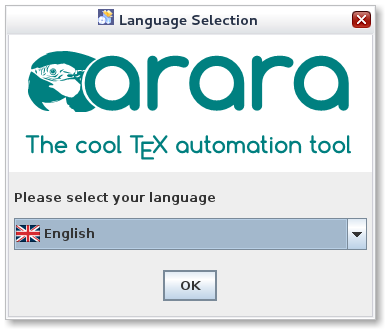
\includegraphics[scale=0.5]{figures/install-langsel.png}
\caption{Language selection screen.}
\label{fig:instlang}
\end{figure}

The installer currently supports six languages: English, German, French, Italian, Spanish, and Brazilian Portuguese. I plan to add more languages to the list in the near feature.

The next screen welcomes you to the installation (Figure~\ref{fig:instwelcome}). There's the application name, the current version, the author's name and e-mail, and the project homepage. We can proceed by clicking the \textit{Next} button. Note that you can quit the installer at any time by clicking the \textit{Quit} button -- please, don't do it; a kitten dies every time you abort the installation\footnote{Of course, this statement is just a joke. No animals were harmed, killed or severely wounded during the making of this user manual. After all, \arara is environmentally friendly.}.

\begin{figure}[p]
\centering
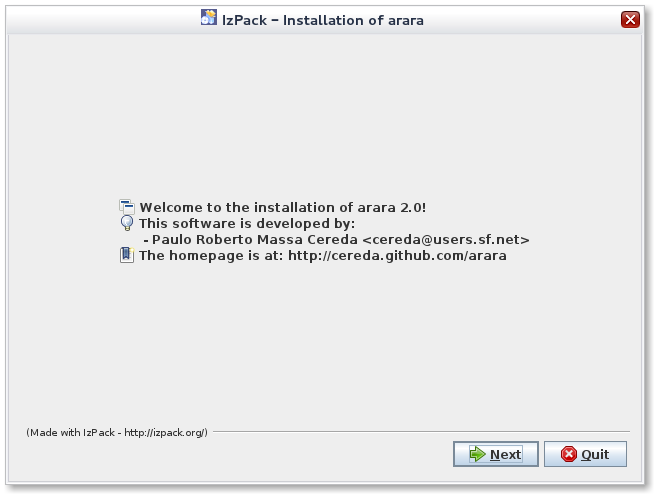
\includegraphics[scale=0.5]{figures/install-welcome.png}
\caption{Welcome screen.}
\label{fig:instwelcome}
\end{figure}

Moving on, the next screen shows the license agreement (Figure~\ref{fig:instlicense}). \arara is licensed under the \href{http://www.opensource.org/licenses/bsd-license.php}{New BSD License}~\cite{bsd:2012}. It's important to observe that the New BSD License has been verified as a GPL-compatible free software license by the Free Software Foundation~\cite{fsf:1985}, and has been vetted as an open source license by the Open Source Initiative~\cite{osi:1998}. The full license is also available in this document (page~\pageref{sec:license}). You need to accept the terms of the license agreement before proceeding.

\begin{figure}[p]
\centering
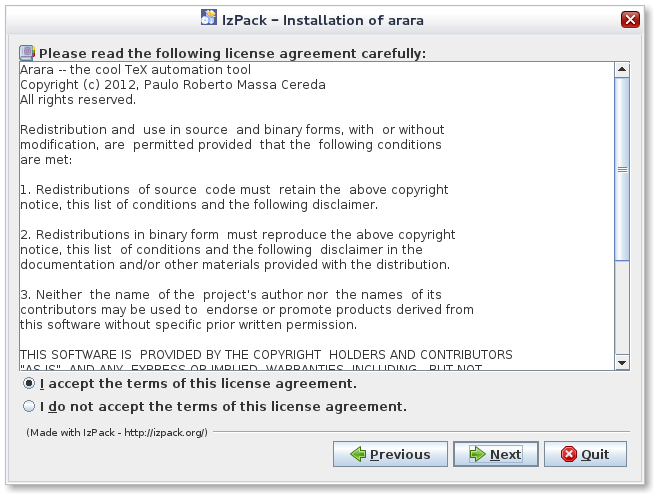
\includegraphics[scale=0.5]{figures/install-license.png}
\caption{License agreement screen.}
\label{fig:instlicense}
\end{figure}

The next screen is probably the most important section of the installation: in here we will choose the packs we want to install (Figure~\ref{fig:instpacks}). All packs are described in Table~\ref{tab:packs}. Note that the grayed packs are required.

\begin{figure}[p]
\centering
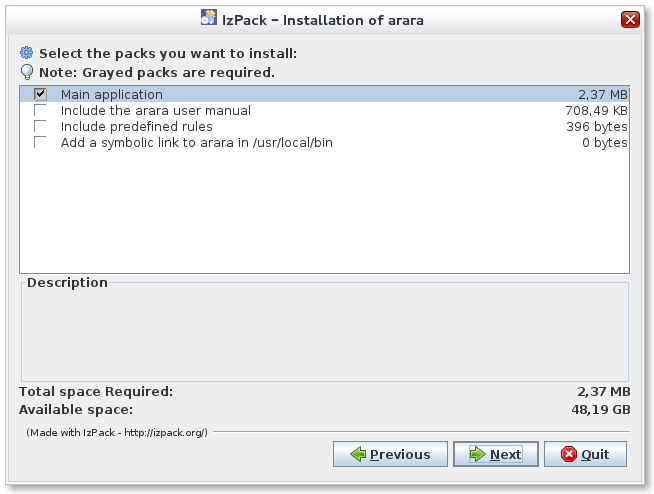
\includegraphics[scale=0.5]{figures/install-packs.png}
\caption{Packs screen.}
\label{fig:instpacks}
\end{figure}

{\renewcommand{\arraystretch}{1.5}
\begin{table}[ht]
\centering
\footnotesize
\begin{tabular}{p{0.30\textwidth}p{0.12\textwidth}p{0.4\textwidth}}
\hline
\textbf{Pack name} & \textbf{OS} & \textbf{Description}\\
\hline
\hline
Main application & All & This pack contains the core application. It also provides an |.exe| wrapper for Windows and a bash file for Unix.\\
\hline
Include the \arara user manual & All & This pack installs this user manual into the |docs/| subdirectory of \arara.\\
\hline
Include predefined rules & All & Of course, \arara has a set of predefined rules for you to start with. If you prefer to write your own rules from scratch, do not select this pack.\\
\hline
Add a symbolic link to \arara in |/usr/local/bin| & Unix & If you ran the installer in privileged mode, a symbolic link to \arara can be created in the |/usr/local/bin| directory. There's no magic here, the installer uses the good old |ln| command.\\
\hline
Add \arara to the system path & Windows & Like the Unix task, \arara can also add itself to the system path. This feature is provided by a Windows script named \href{http://legroom.net/software/modpath}{Modify Path}~\cite{modpath:2012}.\\
\hline
\end{tabular}
\caption{Available packs.}
\label{tab:packs}
\end{table}}

It's very important to mention that all these modifications in the operating system -- the symbolic link creation for Unix or the addition to the path for Windows -- are safely removed when you run the \arara uninstaller. We will talk about it later, in Section~\ref{sec:uninstall}.

In the next screen, we will select the installation path (Figure~\ref{fig:instpath}). The installer will automatically set the default installation path according to the Table~\ref{tab:paths}, but feel free to install \arara in your favorite structure -- even |/opt| or your home folder.

{\renewcommand{\arraystretch}{1.5}
\begin{table}[ht]
\centering
\begin{tabular}{cl}
\hline
\textbf{OS} & \textbf{Default installation path}\\
\hline
\hline
Windows & |C:\Program Files\arara|\\
Unix & |/usr/local/arara|\\
\hline
\end{tabular}
\caption{Default installation paths.}
\label{tab:paths}
\end{table}}

\begin{figure}[p]
\centering
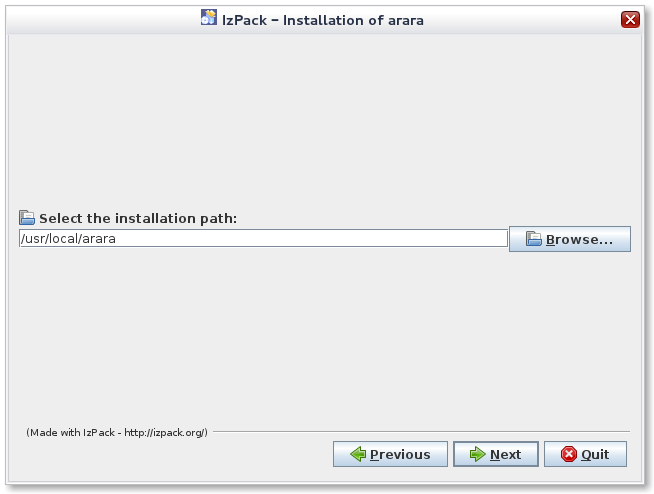
\includegraphics[scale=0.5]{figures/install-path.png}
\caption{Installation path screen.}
\label{fig:instpath}
\end{figure}

After selecting the installation path, the installer will then confirm the creation of the target directory (Figure~\ref{fig:instnewfolder}). We simply click \textit{OK} to accept it. For convenience, the full installation path defined in the installation path screen (Figure~\ref{fig:instpath}) will be referred as |ARARA_HOME| from now on.

\begin{figure}[ht]
\centering
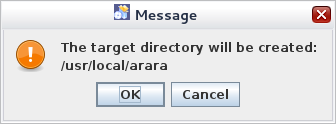
\includegraphics[scale=0.5]{figures/install-pathwarning.png}
\caption{Target directory confirmation.}
\label{fig:instnewfolder}
\end{figure}

Now, just sit back and relax while \arara is being installed (Figure~\ref{fig:instprogress}). All selected packs will be installed accordingly. The post installation tasks -- like creating the symbolic link or adding \arara to the system path -- are performed here as well. If the installation has completed successfully, we will reach the final screen of the installer congratulating us for installing \arara (Figure~\ref{fig:instfinish}).

\begin{figure}[p]
\centering
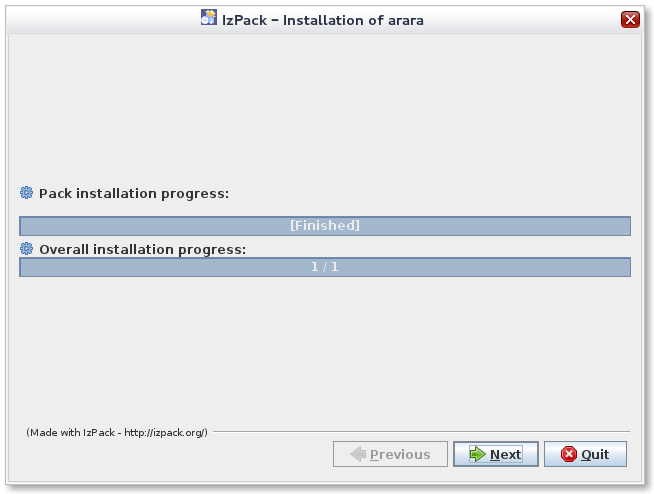
\includegraphics[scale=0.5]{figures/install-progress.png}
\caption{Progress screen.}
\label{fig:instprogress}
\end{figure}

\begin{figure}[p]
\centering
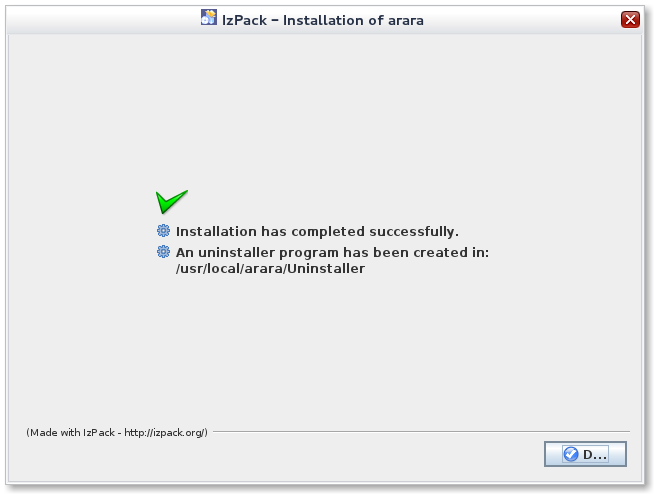
\includegraphics[scale=0.5]{figures/install-finish.png}
\caption{Final screen.}
\label{fig:instfinish}
\end{figure}

The full installation scheme is presented in Figure~\ref{fig:ararastructure}. The directory structure is presented here as a whole; keep in mind that some parts will be omitted according to your operating system and pack selection. For example, the |etc/| subdirectory will only be installed if and only if you are in Windows and the system path pack is selected. Other files are platform-specific, such as |arara.exe| for Windows and the |arara| bash file for Unix.

\begin{figure}[ht]
\centering
\begin{tikzpicture}[grow via three points={one child at (0.5,-0.7) and two children at (0.5,-0.7) and (0.5,-1.4)}, edge from parent path={(\tikzparentnode.south) |- (\tikzchildnode.west)}, anchor=west, font=\ttfamily]
  \node {ARARA\_HOME/}
    child { node {arara.jar}}		
    child { node {arara.exe}}
    child { node {arara}}
    child { node {docs/}
      child { node {arara-usermanual.pdf}}
    }
    child [missing] {}
    child { node {etc/}
      child { node {modpath.exe}}
    }
    child [missing] {}
    child { node {Uninstaller/}
      child { node {uninstaller.jar}}
    }
	child [missing] {}
    child { node {rules/}
	  child { node {plain/}
        child { node {pdflatex.yaml}}
        child { node {\ldots}}
        child { node {xelatex.yaml}}
  	  }
    };
\end{tikzpicture}
\caption{Installation scheme.}
\label{fig:ararastructure}
\end{figure}

That's it, \arara is installed in your operating system. If you opted for the symbolic link creation or the path addition, \arara is already available in your terminal by simply typing |arara|. Have fun!

\section{Manual installation}
\label{sec:manualinstall}

Thankfully, \arara is also very easy to be manually deployed. First of all, we must create the application directory. Feel free to create this directory anywhere in your computer; it can be |C:\arara|, |/opt/arara| or another location of your choice. This procedure is similar to the installation path screen (Figure~\ref{fig:instpath}) from Section~\ref{sec:installer}. Again, for convenience, the full installation path will be referred as |ARARA_HOME| from now on. Although it's not mandatory, try to avoid folders structures with spaces in the path. In any case, \arara can handle such spaces.

After downloading |arara.jar| from the \href{http://github.com/cereda/arara/downloads}{downloads} section of the project repository, let's copy it to the |ARARA_HOME| directory we've created in the previous step. Since |arara.jar| is a self-contained, batteries-included executable Java archive file, \arara is already installed.

In order to run \arara from a manual installation, we should run |java -jar $ARARA_HOME/arara.jar| in the terminal, but that is far from being intuitive. To make our lives easier, we will create a shortcut for this command.

If you are deploying \arara in Windows, there are two methods for creating a shortcut: the first method -- the easiest -- consists of downloading the |arara.exe| wrapper from the \href{http://github.com/cereda/arara/downloads}{downloads} section and copying it to the |ARARA_HOME| directory, in the same level of |arara.jar|. This |.exe| wrapper, provided by \href{http://launch4j.sourceforge.net}{Launch4J}~\cite{launch4j:2005}, wraps |.jar| files in Windows native executables and allows to run them like a regular Windows program.

The second method for creating a shortcut in Windows is to provide a batch file which will call |java -jar $ARARA_HOME/arara.jar| for us. Create a file named |arara.bat| or |arara.cmd| inside the |ARARA_HOME| directory, in the same level of |arara.jar|, and add the content from Code~\ref{code:windows}.

\begin{code}[ht]
\caption{Creating a batch file for \arara in Windows.}
\label{code:windows}
\begin{infobox}
\begin{bash}
@echo off
java -jar "%~dp0\arara.jar" %*
\end{bash}
\end{infobox}
\end{code}

After creating the batch file, add the full |ARARA_HOME| path to the system path. Unfortunately, this manual can't cover the path settings, since it's again a matter of personal taste. I'm sure you can find tutorials on how to add a directory to the system path.

If you are deploying \arara in Linux or Mac, we also need to create a shortcut to |java -jar $ARARA_HOME/arara.jar|. Create a file named |arara| inside the |ARARA_HOME| directory, in the same level of |arara.jar|, and add the content from Code~\ref{code:unix}.

\begin{code}[p]
\caption{Creating a script for \arara in Linux and Mac.}
\label{code:unix}
\begin{infobox}
\begin{bash}
#!/bin/bash
SOURCE="${BASH_SOURCE[0]}"
while [ -h "$SOURCE" ] ; do SOURCE="$(readlink "$SOURCE")"; done
DIR="$( cd "$( dirname "${BASH_SOURCE[0]}" )" && cd -P "$( dirname "$SOURCE" )" && pwd )"
java -jar "$DIR/arara.jar" $*
\end{bash}
\end{infobox}
\end{code}

We now need to add execute permissions for our newly created script through |chmod +x arara|. The |arara| script can be invoked through path addition or symbolic link. I personally prefer to add |ARARA_HOME| to my user path, but a symbolic link creation seems way more robust -- it's what the installer does. Anyway, it's up to you to decide which method you want to use. There's no need to use both.

Once we conclude the manual installation, it's time to check if \arara is working properly. Try running |arara| in the terminal and see if you get the output shown in Code~\ref{code:arararun}.

\begin{code}[p]
\caption{Testing if \arara is working properly.}
\label{code:arararun}
\begin{infobox}
\begin{nolanguage}
$ arara
  __ _ _ __ __ _ _ __ __ _
 / _` | '__/ _` | '__/ _` |
| (_| | | | (_| | | | (_| |
 \__,_|_|  \__,_|_|  \__,_|

Arara 2.0 - The cool TeX automation tool
Copyright (c) 2012, Paulo Roberto Massa Cereda
All rights reserved.

usage: arara [ file [ --log ] [ --verbose ] [ --timeout N ] | --help | --version ]

 -h,--help            print the help message
 -l,--log             generate a log output
 -t,--timeout <arg>   set the execution timeout (in milliseconds)
 -v,--verbose         print the command output
 -V,--version         print the application version
\end{nolanguage}
\end{infobox}
\end{code}

If the terminal doesn't display the \arara logo and usage, please review the manual installation steps. Every step is important in order to make \arara available in your system. You can also try the cross-platform installer. If you still have any doubts, feel free to contact me.

\section{Updating \texorpdfstring{\arara}{arara}}
\label{sec:updating}

If there is a newer version of \arara available in the \href{http://github.com/cereda/arara/downloads}{downloads} section of the project repository, simply download the |arara.jar| file and copy it to the |ARARA_HOME| directory, replacing the current one. No further steps are needed, the newer version is deployed. Try running |arara --version| in the terminal and see if the version shown in the output is equal to the one you have downloaded.

Anyway, for every version, \arara has the proper cross-platform installer available for download in the project repository. You can always uninstall the old \arara setup and install the new one.

\section{Uninstalling \texorpdfstring{\arara}{arara}}
\label{sec:uninstall}

If you want to uninstall \arara, there are two methods available. If you installed \arara through the cross-platform installer, I have good news for you: you only need to run the uninstaller. Now, if \arara was deployed through the manual installation, we might have to remove some links or path additions.

A general Unix-based uninstallation can be triggered by the command presented in Code~\ref{code:uninstall1}. There's also an alternative command presented in Code~\ref{code:uninstall2}.

\begin{code}[ht]
\caption{Running the uninstaller in a Unix-based system -- method 1.}
\label{code:uninstall1}
\begin{infobox}
\begin{bash}
$ sudo java -jar $ARARA_HOME/Uninstaller/uninstaller.jar
\end{bash}
\end{infobox}
\end{code}

\begin{code}[ht]
\caption{Running the uninstaller in a Unix-based system -- method 2.}
\label{code:uninstall2}
\begin{infobox}
\begin{bash}
$ su -c 'java -jar $ARARA_HOME/Uninstaller/uninstaller.jar'
\end{bash}
\end{infobox}
\end{code}

Since Windows doesn't have a similar command to |su| or |sudo|, you need to open the command prompt as administrator and then run the command presented in Code~\ref{code:uninstallwin}. You can right-click the command prompt shortcut and select the ``Run as administrator\ldots'' option.

\begin{code}[ht]
\caption{Running the uninstaller in the Windows command prompt as administrator.}
\label{code:uninstallwin}
\begin{infobox}
\begin{bash}
C:\> java -jar $ARARA_HOME/Uninstaller/uninstaller.jar
\end{bash}
\end{infobox}
\end{code}

The uninstallation process will begin. Hopefully, the first -- and only -- screen of the uninstaller will appear (Figure~\ref{fig:uninstallone}). By the way, if you called the uninstaller through the command line, please do not close the terminal! It might end the all running processes, including our uninstaller.

\begin{figure}[ht]
\centering
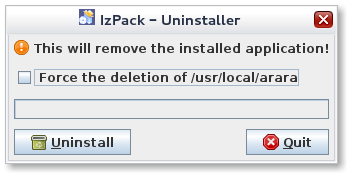
\includegraphics[scale=0.5]{figures/uninstall-welcome.png}
\caption{The uninstaller screen.}
\label{fig:uninstallone}
\end{figure}

There's nothing much to see in the uninstaller. We have an option to force the deletion of the |ARARA_HOME| directory, but that's all. By clicking the \textit{Uninstall} button, the uninstaller will remove the symbolic link or the path entry for \arara from the operating system, if selected during the installation. Then it will erase the |ARARA_HOME| directory (Figure~\ref{fig:uninstalltwo}).

\begin{figure}[ht]
\centering
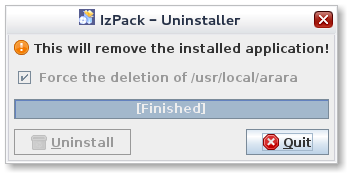
\includegraphics[scale=0.5]{figures/uninstall-finish.png}
\caption{The uninstaller screen, after the execution.}
\label{fig:uninstalltwo}
\end{figure}

Unfortunately, even if you force the deletion of the |ARARA_HOME| directory in Windows, the operating system can't remove the |Uninstaller| subdirectory because the uninstaller was being executed from there. But that's the only trace left. You can safely delete |ARARA_HOME| after running the uninstaller.

If \arara was manually installed, we need to remove the symbolic link reference or the path entry, if any, then delete the |ARARA_HOME| directory. Don't leave any traces of \arara in system directories or configuration files; a broken symbolic link or a wrong path entry might cause trouble in the future.

\section{Integrating \texorpdfstring{\arara}{arara} with \texorpdfstring{\TeX works}{TeXworks}}
\label{sec:texworks}

\arara can be easily integrated with \TeX works~\cite{texworks:2009}, an environment for authoring \TeX\ documents shipped with both \TeX\ Live and MiK\TeX. In this section, we will learn how to integrate \arara and this great cross-platform \TeX\ front-end program.

First of all, make sure \arara is properly installed in your operating system. Thankfully, it's very easy to add a new tool in \TeX works, just open the program and click in \textit{Edit} $\rightarrow$ \textit{Preferences\ldots} to open the preferences screen (Figure~\ref{fig:texworkspref}).

\begin{figure}[pht]
\centering
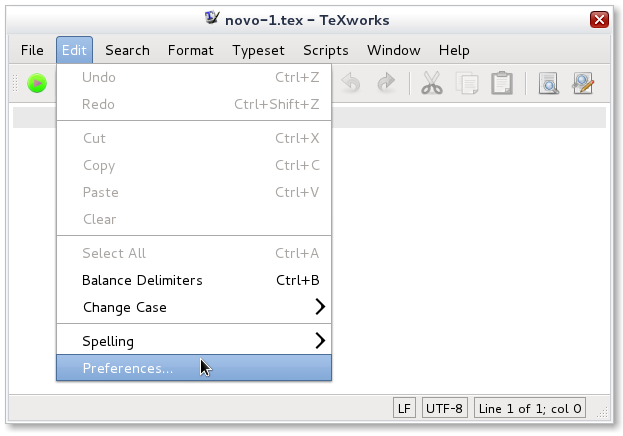
\includegraphics[scale=0.5]{figures/texworks-prefs.png}
\caption{Opening the preferences screen in \TeX works.}
\label{fig:texworkspref}
\end{figure}

The next screen is the \TeX works preferences (Figure~\ref{fig:texworksprefscreen}). There are several tabs available. Navigate to the \textit{Typesetting} tab, which contains two lists: the paths for \TeX\ and related programs, and the processing tools. In the second list -- the processing tools -- click the \textit{Plus (+)} button to add another tool.

\begin{figure}[pht]
\centering
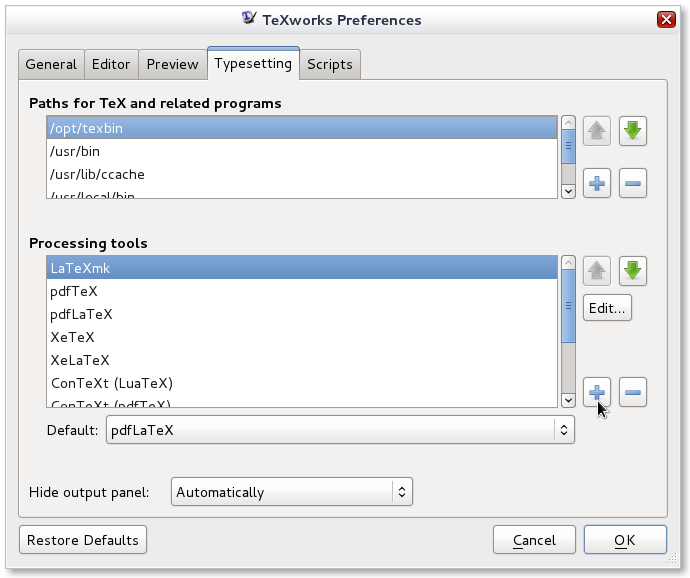
\includegraphics[scale=0.5]{figures/texworks-add.png}
\caption{The \TeX works preferences screen.}
\label{fig:texworksprefscreen}
\end{figure}

We are now in the new tool screen (Figure~\ref{fig:texworksarara}). \TeX works provides an very straightforward interface for adding new tools; we just need to provide the tool name, the executable path, and the parameters. Table~\ref{tab:texworksarara} helps us on what to type in each field. When done, just click \textit{OK} and our new tool will be available.

\begin{figure}[pht]
\centering
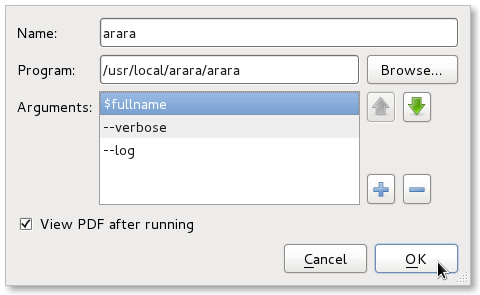
\includegraphics[scale=0.5]{figures/texworks-arara.png}
\caption{The new tool screen.}
\label{fig:texworksarara}
\end{figure}

{\renewcommand{\arraystretch}{1.5}
\begin{table}[pht]
\centering
\footnotesize
\begin{tabular}{p{0.15\textwidth}p{0.25\textwidth}p{0.50\textwidth}}
\hline
\textbf{Field name} & \textbf{Value} & \textbf{Description}\\
\hline
\hline
Name & |arara| & The tool name. You can actually type whatever name your heart desires. This value will be displayed in the compilation profile.\\
\hline
Program & |$ARARA_HOME/arara| & The full executable path. Just browse the filesystem and select the correct \arara path. Observe that symbolic links are resolved to their full targets. For Windows, select the |.exe| wrapper; for Unix, select the bash script.\\
\hline
Arguments & {\renewcommand{\arraystretch}{1}
\begin{tabular}[t]{l}
|$fullname|\\
|--verbose|\\
|--log|
\end{tabular}} & The tool arguments. Note that you need to type one argument at a time, by clicking the \textit{Plus (+)} button. The first argument is a \TeX works variable which will expand to the current filename. The second and third arguments are \arara flags, discussed later, in Chapter~\ref{chap:gettingstarted}.\\
\hline
\end{tabular}
\caption{Configuring \arara in \TeX works.}
\label{tab:texworksarara}
\end{table}}

We are now back to the preferences screen (Figure~\ref{fig:texworksprefscreen}). Hopefully, \arara is in the list of processing tools. Just click \textit{OK} to confirm the new addition. Congratulations, now \arara is available as a compilation profile in \TeX works (Figure~\ref{fig:texworksprofile}).

\begin{figure}[pht]
\centering
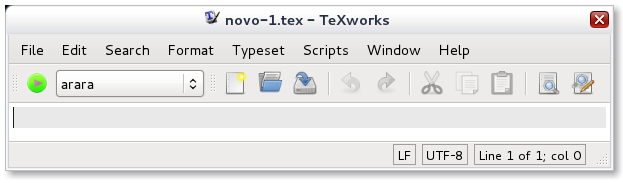
\includegraphics[scale=0.5]{figures/texworks-profile.png}
\caption{Using \arara in the \TeX works compilation profile.}
\label{fig:texworksprofile}
\end{figure}

You can integrate \arara with other \TeX\ editors as well, but sadly their configuration process is far beyond the scope of this humble user manual. However, I'm sure these editors can provide you a step-by-step guide on how to add a new tool or a compilation profile, so you'll be able to use \arara with them. My friend Clemens Niederberger wrote a nice tutorial on how to integrate \arara and Kile, it's surely worth a read~\cite{niederberger:2012}. Happy \TeX ing!

\printbibliography[heading=subbibliography]
% -------------------------------------------------

% Getting started
% -------------------------------------------------
\chapter{Getting started}
\label{chap:gettingstarted}

\epigraph{\emph{Is Batman a scientist?}}{Homer Simpson}

Time for our first contact with \arara! It's important to understand two concepts in which \arara is based on: rules and directives. A \emph{rule} is a formal description of how \arara should handle a certain task. For example, if we want to use |pdflatex| with \arara, we should have a rule for that. Once a rule is defined, \arara automatically provides an access layer to that rule through directives. A \emph{directive} is a special comment in the |.tex| file 
which will tell \arara how it should execute a certain task. A directive can have as many parameters as its corresponding rule has. Don't worry, let's get started with these new concepts.

\section{Rules}
\label{sec:rules}

Do you remember |mydoc.tex| from Code~\ref{code:hellolatex} in page~\pageref{code:hellolatex}? When we tried to mimic |rubber| and run |arara mydoc|, nothing happened. We should tell \arara how it should handle this execution. Let's start with the rules.

A rule is a plain text file written in the YAML format~\cite{yaml:2001}. I opted for this format because it's cleaner and more intuitive to use than other markup 
languages, besides of course being a data serialization standard for all programming languages. As a bonus, the acronym \emph{YAML} rhymes with the word \emph{camel}, so \arara is heavily environmentally friendly.

The rules must be placed in a special subdirectory inside |ARARA_HOME|. The full path for plain \arara rules is |ARARA_HOME/rules/plain|, so feel free to create this directory structure before proceeding with the reading -- well, if you selected the rules pack during the installation, you already have a handful of rules to start with. Wait a minute, what is a plain rule? Easy, it's a rule written using the YAML format. We can also have compiled rules in the form of |.jar| files to be placed inside the |ARARA_HOME/rules/compiled| directory, but I'm almost sure you will never need to write one of them. We will learn how to write compiled rules in Chapter~\ref{chap:writingcompiledrules}. The basic structure of a plain \arara rule is presented in Code~\ref{code:yamlrule}.

\begin{code}[ht]
\caption{\mycmd{makefoo.yaml}, a basic structure of a plain \arara rule.}
\label{code:yamlrule}
\begin{infobox}[innertopmargin=3pt, innerbottommargin=3pt,innerleftmargin=10pt, innerrightmargin=3pt]
\begin{yaml}
<R>!config<A>
<B>identifier:<A> makefoo
<B>name:<A> MakeFoo
<B>command:<A> makefoo <G>@{<A>file<G>}<A>
<B>arguments:<A> <G>[<A><G>]<A>
\end{yaml}
\end{infobox}
\end{code}

The |!config| keyword (line 1) is mandatory and it must be the first line of a plain \arara rule. The following keys are defined:

\begin{description}
\item[identifier] This key (line 2) acts as a unique identifier for the rule. It's highly recommended to use lowercase letters without spaces, accents or punctuation symbols. As a convention, if you have an identifier named |makefoo|, the rule filename must be |makefoo.yaml|.
\item[name] The |name| key (line 3) holds the name of the task. When running \arara, this value will be displayed in the output. In our example, \arara will display |Running MakeFoo| in the output when dealing with this task.
\item[command] This key (line 4) contains the system command to be executed. You can use virtually any type of command, interactive or noninteractive. But beware: if \arara is running in silent mode, which is the default behaviour, an interactive command wich might require the user input will be halted and the execution will fail. Don't dispair, you can use a special |--verbose| flag with \arara in order to interact with such commands -- we will talk about flags in Section~\ref{sec:araraflags}. You probably noticed a strange element |@{file}| in the |command| line: this element is called \emph{orb tag}. For now, just admit they exist. We will come back to them later on, in Section~\ref{sec:orbtags}, I promise.
\item[arguments] The |arguments| key (line 5) denotes a list of arguments for the rule command. In our example, we have an empty list, denoted as |[]|. You can define as many arguments as your command requires.    Please check Code~\ref{code:makebar} for an example of a list of arguments.
\end{description}

For more complex rules, we might want to use arguments. Code~\ref{code:makebar} presents a new rule which makes use of them instead of an empty list as we saw in Code~\ref{code:yamlrule}.

\begin{code}[ht]
\caption{\mycmd{makebar.yaml}, a rule with arguments.}
\label{code:makebar}
\begin{infobox}[innertopmargin=3pt, innerbottommargin=3pt, innerleftmargin=10pt, innerrightmargin=3pt]
\begin{yaml}
<R>!config<A>
<B>identifier:<A> makebar
<B>name:<A> MakeBar
<B>command:<A> makebar <G>@{<A>one<G>}<A> <G>@{<A>two<G>}<A> <G>@{<A>file<G>}<A>
<B>arguments:<A>
<B>- identifier:<A> one
   <B>flag:<A> -i <G>@{<A>value<G>}<A>
<B>- identifier:<A> two
   <B>flag:<A> -j <G>@{<A>value<G>}<A>
\end{yaml}
\end{infobox}
\end{code}

For every argument in the list, we have a |-| mark and the proper indentation. The required keys for an argument are:

\begin{description}
\item[identifier] This key (lines 6 and 8) acts as a unique identifier for the argument. It's highly recommended to use lowercase letters without spaces, accents or 
     punctuation symbols.
\item[flag] The |flag| key (lines 7 and 9) represents the argument value. Note that we have another orb tag in the definition, |@{value}|. We will discuss them later in Section~\ref{sec:orbtags}.
\end{description}

For now, we need to keep in mind that \arara uses rules to tell it how to do a certain task. In the next sections, when more concepts are presented, we will come back to this subject. Just a taste of things to come: directives are mapped to rules through orb tags. Don't worry, I'll explain how things work.

\section{Directives}
\label{sec:directives}

A \emph{directive} is a special comment inserted in the |.tex| file in which you indicate how \arara should behave. You can insert as many directives as you want, and in any position of the |.tex| file. \arara will read the whole file and extract the directives. A directive should be placed in a line of its own, in the form |% arara: <directive>|. There are two types of directives:

\begin{description}
\item[empty directive]  An empty directive, as the name indicates, has only the rule identifier, as we seen in Section~\ref{sec:rules}. Lines 1 and 3 of Code~\ref{code:directiveslatex} show an example of empty directives. Note that you can supress arguments (line 3 in constrast to line 2), but we will see that \arara assumes that you know exactly what you are doing. The syntax for an empty directive is |% arara: makefoo|.
\item[parametrized directive] A parametrized directive has the rule identifier followed by its arguments. Line 2 of Code~\ref{code:directiveslatex} shows an example of a parametrized directive. It's very important to mention that the arguments are mapped by their identifiers and not by their positions. The syntax for a parametrized directive is |% arara: makefoo: { arglist }|. The argument is in the form |arg: value|; a list of arguments and their respective values is separated by comma.
\end{description}

\begin{code}[ht]
\caption{Example of directives in a \mycmd{.tex} file.}
\label{code:directiveslatex}
\begin{infobox}[innertopmargin=3pt, innerbottommargin=3pt, 
                innerleftmargin=10pt, innerrightmargin=3pt]
\begin{latex}
% (*@@*)arara: makefoo
% (*@@*)arara: makebar: { one: hello, two: bye }
% (*@@*)arara: makebar
\documentclass{article}
...
\end{latex}
\end{infobox}
\end{code}

The arguments are defined according to the rule mapped by the directive. For example, the rule |makebar| (Code~\ref{code:makebar}) has a list of two arguments, |one| and |two|. So you can safely write |makebar: { one: hello }|, but trying to map a nonexisting argument with |makebar: { three: hi }| will raise an error.

If you want to disable an \arara directive, there's no need of removing it from the |.tex| file. Simply replace |% arara:| by |% !arara:| and this directive will be ignored. \arara always look for a line that, after removing the leading and trailing spaces, starts with a comment |%| and has the keyword |arara:| in it.

Directives are mapped to rules. In Section~\ref{sec:orbtags} we will learn about orb tags and then revisit rules and directives. I hope the concepts will be clearer 
since we will understand what an orb tag is and how it works. How about a nice cup of coffee?

\section{Orb tags}
\label{sec:orbtags}

When I was planning the mapping scheme, I opted for a templating mechanism. I was looking for flexibility, and the powerful \href{http://mvel.codehaus.org}{MVEL} expression language~\cite{mvel:2012} was perfect for the job. I could extend my mapping plans by using orb tags. An \emph{orb tag} consists of a |@| character followed by braces |{...}| which contain regular MVEL expressions. In particular, \arara uses the |@{}| expression orb, which contains a value expression which will be evaluated to a string, and appended to the output template. For example, the following template |Hello, my name is @{name}| with the |name| variable resolving to |Paulo| will be expanded to the string |Hello, my name is Paulo|. Cool, isn't it?

When mapping rules, every command argument will be mapped to the form |@{identifier}| with value equals to the content of the |flag| key. There are two reserved orb tags, |@{file}| and |@{value}| -- actually, that's not true, there's a third reserved orb tag which plays a very special role in \arara \ -- |@{SystemUtils}| -- but we will talk about it later on. The |@{file}| orb tag refers to the |.tex| filename argument passed to \arara. The extension is removed, so no matter if \arara is called with |arara mydoc.tex| or |arara mydoc|, |@{file}| will be expanded to |mydoc|. The |@{file}| value can be overriden, but we will discuss it later. The second reserved orb tag |@{value}| is expanded to the argument value passed in the directive. If you have |makebar: { one: hello }|, the |flag| key of argument |one| will be expanded from the original definition |-i @{value}| to |-i hello|. Now |@{one}| contains the expanded |flag| value, which is |-i hello|. All arguments tags are expanded in the rule command. If one of them is not defined in the directive, \arara will admit an empty value, so the |command| flag will be expanded to |makebar -i hello mydoc|. The whole procedure is summarized as follows:

\begin{enumerate}
\item \arara processes a file named |mydoc.tex|.
\item A directive |makebar: { one: hello }| is found, so \arara will look up the rule |makebar.yaml| (Code~\ref{code:makebar}) inside the plain rules directory. I should mention that plain rules have precedence over compiled rules, so if you have both |makebar.yaml| and |makebar.jar|, \arara will pick up the first one.
\item The argument |one| is defined and has value |hello|, so the corresponding |flag| key will have the orb tag |@{value}| expanded to |hello|. The new value is now added to the template referenced by the |command| key and then |@{one}| is expanded to |-i hello|.
\item The argument |two| is not defined, so the template referenced by the |command| key has |@{two}| expanded to an empty string.
\item There are no more arguments, so the template referenced by the |command| key now expands |@{file}| to |mydoc|.
\item The final command is now |makebar -i hello mydoc|.
\end{enumerate}

There's a reserved directive key named |files|, which is in fact a list. In case you want to override the default |@{file}| value, use the |files| key, like |makebar: { files: [ thedoc ] }|. This will result in |makebar thedoc| instead of |makebar mydoc|.

If you provide more than one file in the list, \arara will replicate the directive for every file found, so  |makebar: { files: [ a, b, c ] }| will result in three commands: |makebar a|, |makebar b| and |makebar c|.

Before jumping into some practical examples, let's first learn about how to use \arara in the command line. There are some flags that might literally save our lives.

\section{\texorpdfstring{\arara}{arara} in the command line}
\label{sec:araraflags}

\arara has a very simple command line interface. A simple |arara mydoc| does the trick -- provided that |mydoc| has the proper directives. The default behaviour is to run in silent mode, that is, only the name and the execution status of the current task are displayed. The idea of the silent mode is to provide a concise output. Sadly, in some cases, we want to follow the compilation workflow and even interact with a command which requires user input. If you have an interactive command, \arara won't even bother about it: the execution will halt and the command will fail. Well, that's the silent mode. Thankfully, \arara has a set of flags that can change the default behaviour or even enhance the compilation workflow. Table~\ref{tab:araraflags} shows the list of available \arara flags, with both short and long options.

{\renewcommand{\arraystretch}{1.5}
\begin{table}[ht]
\centering
\footnotesize
\begin{tabular}{p{0.1\textwidth}p{0.2\textwidth}p{0.55\textwidth}}
\hline
\textbf{Flag} & & \textbf{Behaviour}\\
\hline
\hline
|-h| & |--help| & This flag prints the help message, as seen in Code~\ref{code:arararun}, and exits the application. If you run |arara| without any flags or a file to process, this is the default behaviour.\\
\hline
|-l| & |--log| & The |--log| flag enables the logging feature of \arara. All streams from all commands will be logged and, at the end of the execution, an |arara.log| file will be generated. The logging feature is discussed in Chapter~\ref{chap:logging}.\\
\hline
|-t n| & |--timeout n| & This flag sets an execution timeout for every task. If the timeout is reached before the task ends, \arara will kill it and interrupt the processing. The $n$ value is expressed in milliseconds. \\
\hline
|-v| & |--verbose| & The |--verbose| flag enables all streams to be flushed to the terminal -- exactly the opposite of the silent mode. This flag also allows user input if the current command requires so. The user input interaction is possible thanks to the amazing Apache Commons Exec library~\cite{exec:2010}.\\
\hline
|-V| & |--version| & This flag, as the name indicates, prints the current \arara version and exits the application.\\
\hline
\end{tabular}
\caption{The list of available \arara flags.}
\label{tab:araraflags}
\end{table}}

\arara can recognize three types of files based on their extension: |.tex|, |.dtx| and |.ltx|. Other extensions are not recognized, so make sure to have the correct extension in your \TeX\ files.

The combination of flags is very useful to enhance the \TeX\ experience. They can provide nice features for integrating \arara with \TeX\ editors, like \TeX works in Section~\ref{sec:texworks}. Note that both |--log| and |--verbose| flags were used -- we can have both terminal and file output at the same time without any cost.

\section{Examples}
\label{sec:examples}

Now that we know about rules, directives, orb tags, and command line flags, it's time to come up with some examples. I know it's not trivial to understand how \arara works, but I'm sure the examples will help with the concepts. Please note that there might have platform-specific rules, so double-check the commands before running them -- actually, don't worry, \arara has a card up its sleeve.

\subsection{\texorpdfstring{\hologo{pdfLaTeX}}{PDFLaTeX}}
\label{sub:pdflatex}

Our first example is to add support to \hologo{pdfLaTeX}. My first attempt to write this rule is presented in Code~\ref{code:pdflatexone}.

\begin{code}[ht]
\caption{\mycmd{pdflatex.yaml}, first attempt.}
\label{code:pdflatexone}
\begin{infobox}[innertopmargin=3pt, innerbottommargin=3pt, innerleftmargin=10pt, innerrightmargin=3pt]
\begin{yaml}
<R>!config<A>
<B>identifier:<A> pdflatex
<B>name:<A> PDFLaTeX
<B>command:<A> pdflatex <G>@{<A>file<G>}<A>.tex
<B>arguments:<A> <G>[<A><G>]<A>
\end{yaml}
\end{infobox}
\end{code}

So far, so good. The |command| flag has the |pdflatex| program and the |@{file}| orb tag. Remember that |@{file}| is expanded to the filename without the extension. Now we can add the |pdflatex| directive to our |.tex| file, as we can see in Code~\ref{code:helloexampleone}.

\begin{code}[ht]
\caption{\mycmd{helloworld.tex}}
\label{code:helloexampleone}
\begin{infobox}[innertopmargin=3pt, innerbottommargin=3pt, innerleftmargin=10pt, innerrightmargin=3pt]
\begin{latex}
% (*@@*)arara: pdflatex
\documentclass{article}

\begin{document}

Hello world.

\end{document}
\end{latex}
\end{infobox}
\end{code}

It's just a matter of calling |arara helloworld| (you can also provide the |.tex| extension by calling |arara helloworld.tex|, after all the extension will be removed anyway) and \arara will process our file, according to the Code~\ref{code:araraoutputone}.

\begin{code}[ht]
\caption{\arara output for \mycmd{pdflatex}.}
\label{code:araraoutputone}
\begin{infobox}
\begin{bash}
$ arara helloworld
  __ _ _ __ __ _ _ __ __ _
 / _` | '__/ _` | '__/ _` |
| (_| | | | (_| | | | (_| |
 \__,_|_|  \__,_|_|  \__,_|

Running PDFLaTeX... SUCCESS
\end{bash}
\end{infobox}
\end{code}

Great, our first rule works like a charm. Once we define a rule, the directive is automatically available for us to call it as many times as we want. What if we make this rule better? Consider the following situation:

\begin{quotation}
\noindent Sometimes, we need to use |\write18| to call a package that makes use of it (for example, |minted|). It's very dangerous to enable shell escape globally, but changing the |pdflatex| call every time we need it sounds boring.
\end{quotation}

\arara has a special treatment for cases like this. In the early stages of development, \arara was able to handle boolean values. Entries with |true| or |false|, |on| or |off|, |yes| and |no| were mapped to boolean values. If you wanted to use |yes| as text, you could explicitly tell \arara that the value was a string by enclosing it with single or double quotes, |'yes'| or |"yes"|. In my humble opinion, it was a good design at first, but it opened a dangerous pitfall: if a certain mapping was expecting 
a boolean, but another value was received, the result was automatically resolved to |true|. We have enough problems of \arara itself giving us enough rope, so I decided to consider every argument value as string. No big deal, we can still mimic a boolean behaviour, as we will see in our next attempt.

We will rewrite our |pdflatex| rule to include a flag for shell escape. Another cool feature will be presented now, as we can see in the new rule shown in Code~\ref{code:pdflatextwo}.

\begin{code}[ht]
\caption{\mycmd{pdflatex.yaml}, second attempt.}
\label{code:pdflatextwo}
\begin{infobox}[innertopmargin=3pt, innerbottommargin=3pt, innerleftmargin=10pt, innerrightmargin=3pt]
\begin{yaml}
<R>!config<A>
<B>identifier:<A> pdflatex
<B>name:<A> PDFLaTeX
<B>command:<A> pdflatex <G>@{<A>shell<G>}<A> <G>@{<A>file<G>}<A>.tex
<B>arguments:<A>
<B>- identifier:<A> shell
   <B>flag:<A> '<G>@{<A>value == "yes" ? "--shell-escape" : "--no-shell-escape" <G>}<A>'
\end{yaml}
\end{infobox}
\end{code}

Orb tags allow evaluation inside the tag block! Line 7 from Code~\ref{code:pdflatextwo} makes use of the ternary operator |?:| which defines a conditional expression. In the first part of the evaluation, we check if |value| is equal to the string |"yes"|. If so, |"--shell-escape"| is defined as the result of the operation. If the conditional expression is false, |"--no-shell-escape"| is set instead.

What if you want to allow |true| and |on| as valid options as well? We can easily rewrite our orb tag to check for additional values. It's also possible to invoke some string methods on orb tags, like |toLowerCase|. A third attempt is presented in Code~\ref{code:pdflatexthree}. The |toLowerCase| method was added to allow entries like |Yes|, |yEs| and other case combinations. Although \arara can support cases in arguments and values, I recommend you to stick with lowercase entries. By the way, for more complex orb tag schemes, it's important to enclose the orb tags with either single or double quotes. Of course, if you use single quotes to enclose the orb tags, use 
double quotes for internal evaluations, and vice versa.

\begin{code}[ht]
\caption{\mycmd{pdflatex.yaml}, third attempt.}
\label{code:pdflatexthree}
\begin{infobox}[innertopmargin=3pt, innerbottommargin=3pt, innerleftmargin=10pt, innerrightmargin=3pt]
\begin{yaml}
<R>!config<A>
<B>identifier:<A> pdflatex
<B>name:<A> PDFLaTeX
<B>command:<A> pdflatex <G>@{<A>shell<G>}<A> <G>@{<A>file<G>}<A>.tex
<B>arguments:<A>
<B>- identifier:<A> shell
   <B>flag:<A> '<G>@{<A>value.toLowerCase() == "yes" || value.toLowerCase() == "true" || value.toLowerCase() == "on" ? "--shell-escape" : "--no-shell-escape" <G>}<A>'
\end{yaml}
\end{infobox}
\end{code}

With this new rule, it's now easy to enable the shell escape option in |pdflatex|. Simply go with the directive |pdflatex: { shell: yes }|. You can also use |true| or |on| instead of |yes|. Any other value for |shell| will disable the shell escape option. It's important to observe that \arara directives have no mandatory arguments. If you want to add a dangerous option like |--shell-escape|, consider calling it as an argument with a proper check and rely on a safe state for the argument fallback.

\subsection{MakeIndex}
\label{sub:makeindex}

For the next example, we will create a rule for MakeIndex. To be honest, although |makeindex| has a lot of possible arguments, I only use the |-s| flag once in a while. Code~\ref{code:makeindexone} shows our first attempt of writing this rule.

\begin{code}[ht]
\caption{\mycmd{makeindex.yaml}, first attempt.}
\label{code:makeindexone}
\begin{infobox}[innertopmargin=3pt, innerbottommargin=3pt, innerleftmargin=10pt, innerrightmargin=3pt]
\begin{yaml}
<R>!config<A>
<B>identifier:<A> makeindex
<B>name:<A> MakeIndex
<B>command:<A> makeindex <G>@{<A>style<G>}<A> <G>@{<A>file<G>}<A>.idx
<B>arguments:<A>
<B>- identifier:<A> style
   <B>flag:<A> -s <G>@{<A>value<G>}<A>
\end{yaml}
\end{infobox}
\end{code}

As a follow-up to our first attempt, we will now add support for the |-g| flag that employs German word ordering in the index. Since this flag is basically a switch, we can borrow the same tactic used for enabling shell escape in the |pdflatex| rule from Code~\ref{code:pdflatexthree}. The new rule is presented in Code~\ref{code:makeindextwo}.

\begin{code}[ht]
\caption{\mycmd{makeindex.yaml}, second attempt.}
\label{code:makeindextwo}
\begin{infobox}[innertopmargin=3pt, innerbottommargin=3pt, innerleftmargin=10pt, innerrightmargin=3pt]
\begin{yaml}
<R>!config<A>
<B>identifier:<A> makeindex
<B>name:<A> MakeIndex
<B>command:<A> makeindex <G>@{<A>german<G>}<A> <G>@{<A>style<G>}<A> <G>@{<A>file<G>}<A>.idx
<B>arguments:<A>
<B>- identifier:<A> style
   <B>flag:<A> -s <G>@{<A>value<G>}<A>
<B>- identifier:<A> german
   <B>flag:<A> '<G>@{<A>value.toLowerCase() == "yes" || value.toLowerCase() == "true" || value.toLowerCase() == "on" ? "-g" : "" <G>}<A>'
\end{yaml}
\end{infobox}
\end{code}

The new |makeindex| rule presented in Code~\ref{code:makeindextwo} looks good. We can now test the compilation workflow with an example. Consider a file named |helloindex.tex| which has a few index entries for testing purposes, presented in Code~\ref{code:examplemakeindex}. As usual, I'll present my normal workflow, that involves calling |pdflatex| two times to get references right, one call to |makeindex| and finally, a last call to |pdflatex|. Though there's no need of calling |pdflatex| two times in the beginning, I'll keep that as a good practice from my side.

\begin{code}[ht]
\caption{\mycmd{helloindex.tex}}
\label{code:examplemakeindex}
\begin{infobox}[innertopmargin=3pt, innerbottommargin=3pt, innerleftmargin=10pt, innerrightmargin=3pt]
\begin{latex}
% (*@@*)arara: pdflatex
% (*@@*)arara: pdflatex
% (*@@*)arara: makeindex
% (*@@*)arara: pdflatex
\documentclass{article}

\usepackage{makeidx}

\makeindex

\begin{document}

Hello world\index{Hello world}.

Goodbye world\index{Goodbye world}.

\printindex

\end{document}
\end{latex}
\end{infobox}
\end{code}

By running |arara helloindex| or |arara helloindex.tex| in the terminal, we will obtain the same output from Code~\ref{code:araramakeexample}. The execution order is defined by the order of directives in the |.tex| file. If any command fails, \arara halts at that position and nothing else is executed.

You might ask how \arara knows if the command was successfully executed. The idea is quite simple: good programs like |pdflatex| make use of a concept known as exit status. In short, when a program had a normal execution, the exit status is zero. Other values are returned when an abnormal execution happened. When |pdflatex| successfully compiles a |.tex| file, it returns zero, so \arara intercepts this number. Again, it's a good practice to make command line applications return a proper exit status according to the execution flow, but beware: you might find applications or shell commands that don't feature this control (in the worst case, the returned value is always zero). \arara relies on the awesome \href{http://commons.apache.org/exec/}{Apache Commons Exec} library to provide the system calls.

\begin{code}[!ht]
\caption{Running \mycmd{helloindex.tex}.}
\label{code:araramakeexample}
\begin{infobox}
\begin{bash}
$ arara helloindex
  __ _ _ __ __ _ _ __ __ _
 / _` | '__/ _` | '__/ _` |
| (_| | | | (_| | | | (_| |
 \__,_|_|  \__,_|_|  \__,_|

Running PDFLaTeX... SUCCESS
Running PDFLaTeX... SUCCESS
Running MakeIndex... SUCCESS
Running PDFLaTeX... SUCCESS
\end{bash}
\end{infobox}
\end{code}

According to the terminal output shown in Code~\ref{code:araramakeexample}, \arara executed all the commands successfully. In Chapter~\ref{chap:logging} we will learn more about how \arara works with commands and how to get their streams for a more detailed analysis.

\subsection{Bibliography}
\label{sub:bibliography}

For the next example, we will write a rule for both \hologo{BibTeX} and \hologo{biber}. Instead of writing two rules -- one for each command -- I'll show how we can use conditional expressions and run different commands in a single rule. The common scenario is to have each tool mapped to its own rule, but as we can see, rules are very flexible. Let's see how \arara handles this unusual |bibliography| rule presented in Code~\ref{code:bibone}.

\begin{code}[ht]
\caption{\mycmd{bibliography.yaml}}
\label{code:bibone}
\begin{infobox}[innertopmargin=3pt, innerbottommargin=3pt, innerleftmargin=10pt, innerrightmargin=3pt]
\begin{yaml}
<R>!config<A>
<B>identifier:<A> bibliography
<B>name:<A> Bibliography
<B>command:<A> '<G>@{<A>engine.toLowerCase() == "biber" ? "biber" : "bibtex" <G>}<A> <G>@{<A>args<G>}<A> <G>@{<A>file<G>}<A>'
<B>arguments:<A>
<B>- identifier:<A> engine
   <B>flag:<A> '<G>@{<A>value<G>}<A>'
<B>- identifier:<A> args
   <B>flag:<A> '<G>@{<A>value<G>}<A>'
\end{yaml}
\end{infobox}
\end{code}

The |bibliography| rule is quite simple, actually. If no |engine| is provided in the |bibliography| directive, the conditional expression will evaluate to false and the result will be expanded to the fallback |bibtex| value. Otherwise, if the |engine| parameter is set to |biber| -- and only this value -- the rule will expand the result to |biber|. Note that |file| will be expanded to the |.tex| filename without the extension -- this setup ensures that both |bibtex| and |biber| will work, since they use different file extensions. Code~\ref{code:examplebib} presents only the header of our |biblio.tex| file using the new |bibliography| directive. Other options are shown in Table~\ref{tab:biblio}.

\begin{code}[ht]
\caption{\mycmd{biblio.tex}}
\label{code:examplebib}
\begin{infobox}[innertopmargin=3pt, innerbottommargin=3pt, innerleftmargin=10pt, innerrightmargin=3pt]
\begin{latex}
% (*@@*)arara: pdflatex
% (*@@*)arara: bibliography
% (*@@*)arara: pdflatex
\documentclass{article}
...
\end{latex}
\end{infobox}
\end{code}

{\renewcommand{\arraystretch}{1.5}
\begin{table}[ht]
\centering
\footnotesize
\begin{tabular}{p{0.3\textwidth}p{0.55\textwidth}}
\hline
\textbf{Directive} & \textbf{Behaviour}\\
\hline
\hline
\mycmd{bibliography: \{ engine: bibtex \}} & This directive sets the |engine| parameter to |bibtex|, which will expand the command to |bibtex| in the rule. Note that any value other than |biber| will expand the command to |bibtex|. \\
\hline
\mycmd{bibliography: \{ engine: biber \}} &  This directive sets the |engine| parameter to |biber|, which will expand the command to |biber| in the rule. This is the only possible value that will set |biber| as the rule command.\\
\hline
\mycmd{bibliography: \{ engine: bibtex, args: '-min-crossrefs=2' \}} & This directive sets the |engine| parameter to |bibtex| and also provides an argument to the command. Note that the |args| value is specific to |bibtex| -- using this argument value with |biber| will surely raise an error.\\
\hline
\mycmd{bibliography: \{ engine: biber, args: '{-}{-}sortcase=true' \}} & This directive sets the |engine| parameter to |biber| and also provides an argument to the command. Note that the |args| value is specific to |biber| -- using this argument value with |bibtex| will surely raise an error.\\
\hline
\end{tabular}
\caption{Other directive options for \mycmd{bibliography}.}
\label{tab:biblio}
\end{table}}

It's important to note that |bibtex| and |biber| differ in their flags, so I used a global |args| parameter. It is recommended to enclose the |args| value with single or double quotes. Use this parameter with great care, since the values differ from tool to tool. The output is presented in Code~\ref{code:ararabib}.

\begin{code}[!ht]
\caption{Running \mycmd{biblio.tex}.}
\label{code:ararabib}
\begin{infobox}
\begin{bash}
$ arara biblio
  __ _ _ __ __ _ _ __ __ _
 / _` | '__/ _` | '__/ _` |
| (_| | | | (_| | | | (_| |
 \__,_|_|  \__,_|_|  \__,_|

Running PDFLaTeX... SUCCESS
Running Bibliography... SUCCESS
Running PDFLaTeX... SUCCESS
\end{bash}
\end{infobox}
\end{code}

According to the terminal output shown in Code~\ref{code:ararabib}, \arara executed all the commands successfully. A friendly warning: this rule is very powerful because of its flexibility, but the syntax -- specially the conditional expression and the expansion tricks -- might mislead the user. My advice is to exhaustively test the rules before deploying them into production. After all, better be safe than sorry.

\section{Writing cross-platform rules}
\label{sec:crossrules}

When I wrote \arara, one of my goals was to provide a cross-platform tool which behaves exactly the same on every single operating system. Similarly, the rules also follow the same idea, but sadly that's not always possible. After all, at some point, commands are bounded to the underlying operating system.

A rule that call |pdflatex|, for example, is easy to maintain; you just need to ensure there's an actual |pdflatex| command available in the operating system -- in the worst case, \arara warns about a nonexisting command. But there are cases in which you need to call system-specific commands. You could write two or three rules for the same task, say |makefoowin|, |makefoolinux|, and |makefoomac|, but this approach is not intuitive. Besides, if you share documents between operating systems, you'd have to also change the respective directive in your |.tex| file in order to reflect which operating system you are on.

Thankfully, there's a better solution for writing cross-platform rules which require system-specific commands. In Section~\ref{sec:orbtags}, I mentioned about a special orb tag called |@{SystemUtils}| -- it's now time to unveil its power. This orb tag is available for all rules and maps the |SystemUtils| class from the amazing Apache Commons Lang library~\cite{lang:2001}. In other words, we have access to all methods and properties from that class.

Even though we have access to all public methods of the |SystemUtils| class, I believe we won't need to use them -- the available properties are far more useful for us. Table~\ref{tab:properties} shows the most relevant properties for our context. The \href{http://commons.apache.org/lang/api/org/apache/commons/lang3/SystemUtils.html}{Apache Commons Lang documentation} contains the full class description.

{\renewcommand{\arraystretch}{1.5}
\begin{table}[hpt]
\centering
\footnotesize
\begin{tabular}{lp{0.6\textwidth}}
\hline
\textbf{Property} & \textbf{Description}\\
\hline
\hline
|IS_OS_AIX| & True if this is AIX.\\
|IS_OS_FREE_BSD| & True if this is FreeBSD.\\
|IS_OS_HP_UX| & True if this is HP-UX.\\
|IS_OS_IRIX| & True if this is Irix.\\
|IS_OS_LINUX| & True if this is Linux.\\
|IS_OS_MAC| & True if this is Mac.\\
|IS_OS_MAC_OSX| & True if this is Mac.\\
|IS_OS_NET_BSD| & True if this is NetBSD.\\
|IS_OS_OPEN_BSD| & True if this is OpenBSD.\\
|IS_OS_OS2| & True if this is OS/2.\\
|IS_OS_SOLARIS| & True if this is Solaris.\\
|IS_OS_SUN_OS| & True if this is Sun OS.\\
|IS_OS_UNIX| & True if this is a Unix-like system, as in any of AIX, HP-UX, Irix, Linux, Mac~OS~X, Solaris or Sun OS.\\
|IS_OS_WINDOWS| & True if this is Windows.\\
|IS_OS_WINDOWS_2000| & True if this is Windows 2000.\\
|IS_OS_WINDOWS_2003| & True if this is Windows 2003.\\
|IS_OS_WINDOWS_2008| & True if this is Windows 2008.\\
|IS_OS_WINDOWS_7| & True if this is Windows 7.\\
|IS_OS_WINDOWS_95| & True if this is Windows 95.\\
|IS_OS_WINDOWS_98| & True if this is Windows 98.\\
|IS_OS_WINDOWS_ME| & True if this is Windows ME.\\
|IS_OS_WINDOWS_NT| & True if this is Windows NT.\\
|IS_OS_WINDOWS_VISTA| & True if this is Windows Vista.\\
|IS_OS_WINDOWS_XP| & True if this is Windows XP.\\
\hline
\end{tabular}
\caption{Most relevant properties of \mycmd{SystemUtils}.}
\label{tab:properties}
\end{table}}

Every time we want to call any of the available properties presented in Table~\ref{tab:properties}, we just need to use the |SystemUtils.PROPERTY| syntax, check the corresponding value through conditional expressions and define commands or arguments according to the underlying operating system.

\subsection{Cleaning temporary files}
\label{sub:clean}

Let's go back to our examples and add a new plain rule featuring the new |@{SystemUtils}| orb tag, introduced in Section~\ref{sec:crossrules}. Right after running |arara helloindex| successfully (Code~\ref{code:araramakeexample}), we now have as a result a new |helloindex.pdf| file, but also a lot of auxiliary files, as we can see in Code~\ref{code:lsone}.

\begin{code}[ht]
\caption{List of all files after running \mycmd{arara helloindex}.}
\label{code:lsone}
\begin{infobox}
\begin{bash}
$ ls
helloindex.aux  helloindex.ilg  helloindex.log  helloindex.tex
helloindex.idx  helloindex.ind  helloindex.pdf
\end{bash}
\end{infobox}
\end{code}

What if we write a new |clean| rule to remove all the auxiliary files? The idea is to use |rm| to remove each one of them. For now, let's stick with a system-specific rule -- don't worry, we will improve this rule later on.

Since we want our rule to be generic enough, it's now a good opportunity to introduce the use of the reserved directive key |files|, first seen in Section~\ref{sec:orbtags}. This special key is a list that overrides the default |@{file}| value and replicates the directive for every element in the list. I'm sure this will be the easiest rule we've written so far. The |clean| rule is presented in Code~\ref{code:cleanone}.

\begin{code}[ht]
\caption{\mycmd{clean.yaml}, first attempt.}
\label{code:cleanone}
\begin{infobox}[innertopmargin=3pt, innerbottommargin=3pt, innerleftmargin=10pt, innerrightmargin=3pt]
\begin{yaml}
<R>!config<A>
<B>identifier:<A> clean
<B>name:<A> CleaningTool
<B>command:<A> rm -f <G>@{<A>file<G>}<A>
<B>arguments:<A> <G>[<A><G>]<A>
\end{yaml}
\end{infobox}
\end{code}

Note that the command |rm| has a |-f| flag. As mentioned before, commands return an exit status after their calls. If we try to remove a nonexisting file, |rm| will complain and return a value different than zero. This will make \arara halt and print a big ``failure'' on screen, since a non-zero exit status is considered an abnormal execution. If we provide the |-f| flag, |rm| will not complain of a nonexisting file, so we won't be bothered for this trivial task.

Now we need to add the new |clean| directive to our |helloindex.tex| file (Code~\ref{code:examplemakeindex}). Of course, |clean| will be the last directive, since it will only be reachable if everything executed before was returned with no errors. The new header of |helloindex.tex| is presented in Code~\ref{code:examplemakeindextwo}.

\begin{code}[ht]
\caption{\mycmd{helloindex.tex} with the new \mycmd{clean} directive.}
\label{code:examplemakeindextwo}
\begin{infobox}[innertopmargin=3pt, innerbottommargin=3pt, innerleftmargin=10pt, innerrightmargin=3pt]
\begin{latex}
% (*@@*)arara: pdflatex
% (*@@*)arara: pdflatex
% (*@@*)arara: makeindex
% (*@@*)arara: pdflatex
% (*@@*)arara: clean: { files: [ helloindex.aux, helloindex.idx, helloindex.ilg, helloindex.ind, helloindex.log ] }
\documentclass{article}
...
\end{latex}
\end{infobox}
\end{code}

The reserved directive key |files| has five elements, so the |clean| rule will be replicated five times with the orb tag |@{file}| being expanded to each element. If you wish, you can also evaluate the value through conditional expression, as we did before with the other rules. In my opinion, I don't think it's necessary for this particular rule.

Time to run |arara helloindex| again and see if our new |clean| rule works! Code~\ref{code:araramakeexampletwo} shows both \arara execution and directory listing. We expect to find only our source |helloindex.tex| and the resulting |helloindex.pdf| file.

\begin{code}[htp]
\caption{Running \texttt{helloindex.tex} with the new \texttt{clean} rule.}
\label{code:araramakeexampletwo}
\begin{infobox}
\begin{bash}
$ arara helloindex
  __ _ _ __ __ _ _ __ __ _ 
 / _` | '__/ _` | '__/ _` |
| (_| | | | (_| | | | (_| |
 \__,_|_|  \__,_|_|  \__,_|

Running PDFLaTeX... SUCCESS
Running PDFLaTeX... SUCCESS
Running MakeIndex... SUCCESS
Running PDFLaTeX... SUCCESS
Running CleaningTool... SUCCESS
Running CleaningTool... SUCCESS
Running CleaningTool... SUCCESS
Running CleaningTool... SUCCESS
Running CleaningTool... SUCCESS
$ ls
helloindex.pdf  helloindex.tex
\end{bash}
\end{infobox}
\end{code}

Great, the |clean| rule works like a charm! But we have a big issue: if we try to use this rule in Windows, it doesn't work -- after all, |rm| is not a proper Windows command. Worse, replacing |rm| by the equivalent |del| won't probably work. Commands like |del| must be called in the form |cmd /c del|. Should we write another system-specific rule, say, |cleanwin|? Of course not, there's a very elegant way to solve this issue: the |@{SystemUtils}| orb tag.

The idea is very simple: we check if \arara is running in a Windows operating system; if true, we set the command to |cmd /c del|, or |rm -f| otherwise. The new version of our |clean| rule is presented in Code~\ref{code:cleantwo}.

\begin{code}[ht]
\caption{\mycmd{clean.yaml}, second attempt.}
\label{code:cleantwo}
\begin{infobox}[innertopmargin=3pt, innerbottommargin=3pt, innerleftmargin=10pt, innerrightmargin=3pt]
\begin{yaml}
<R>!config<A>
<B>identifier:<A> clean
<B>name:<A> CleaningTool
<B>command:<A> '<G>@{<A>SystemUtils.IS_OS_WINDOWS ? "cmd /c del" : "rm -f" <G>}<A> <G>@{<A>file<G>}<A>'
<B>arguments:<A> <G>[<A><G>]<A>
\end{yaml}
\end{infobox}
\end{code}

There we go, our first cross-platform rule! There's no need of writing a bunch of system-specific rules; only one cross-platform rule is enough. We know that the |clean| rule will work as expected in every operating system, even if the task to be performed relies on system-specific commands. With cross-platform rules, we are able to write cleaner and more concise code.

A friendly warning: note that the |clean| rule is expecting |@{file}| to be overriden, since we rely on the reserved directive key |files|. If by any chance this rule is called without the |files| directive key, that is, an empty directive |% arara: clean|, I have very bad news to you: the rule will be expanded to |rm -f mydoc.tex| and your |.tex| file will be gone! Do you remember what I said in the prologue? \arara gives you enough rope. In other words, \emph{you} will be responsible for how \arara behaves and all the consequences from your actions. After all, freedom always comes at a cost. Again, my advice: make sure to exhaustively test your rules before putting them into production. You can also refer to Chapter~\ref{chap:logging} to learn more about tracking command expansions.

\printbibliography[heading=subbibliography]
% -------------------------------------------------

% When something goes wrong
% -------------------------------------------------
\chapter{Logging}
\label{chap:logging}

\epigraph{\emph{Don't panic!}}{From The Hitchhiker's\\ Guide to the Galaxy}

One of \arara's goals is to reduce the verbosity of commands. Though the extensive output might contain relevant information about the execution process, in most of the cases it is simply to much stuff going on for us to follow. Besides, commands like |pdflatex| generate a proper |.log| file for us to check how things went. \arara's minimalist approach only informs us about the execution status: ``success'' or ``failure''. When things go terribly wrong, we need to rely on more than this status. We should ask \arara to keep track of the execution plan for us.

\section{\texorpdfstring{\arara}{arara} messages}
\label{sec:araramessages}

\arara messages are the first type of feedback provided by \arara. These messages are basically related to rules and directives. Bad syntax, nonexisting rules, malformed directives, wrong expansion, \arara tries to tell you what went wrong. Those messages are usually associated with errors. I tried to include useful messages, like telling in which directive and line an error ocurred, or that a certain rule does not exist or has an incorrect format. \arara also checks if a command is valid. If you try to call a rule that executes a nonexisting |makefoo| command, \arara will complain about it.

These messages usually cover the events that can happen during the preprocessing phase. Don't panic, \arara will tell you what happened. Of course, an error halts the execution, so we need to fix the reported issue before proceeding. Note that \arara can also complain about nonexisting commands -- in this case, the error will be raised in runtime, since it's an underlying operating system dependency.

\section{Getting the command output}
\label{sec:logging}

Another way of looking for an abnormal behaviour is to read the proper |.log| file. Unfortunately, not every command emits a report of its execution and, even if the command generates a |.log| file, multiple runs would overwrite the previous reports and we would have only the last call. \arara provides a more consistent way of monitoring commands and their own behaviour through a global |.log| file that holds every single bit of information. You can enable the logging feature by adding either the 
|--log| or |-l| flags to the |arara| application.

Before we continue, I need to explain about standard streams, since they constitute an important part of the generated |.log| file by \arara. Wikipedia~\cite{streams:2012} has a nice definition of them:

\begin{quotation}
\noindent ``In computer programming, standard streams are preconnected input and output channels between a computer program and its environment (typically a text terminal) when it begins execution. The three \textsc{i/o} connections are called standard input (|stdin|), standard output (|stdout|) and standard error (|stderr|).''
\end{quotation}

Basically, the operating system provides two streams directed to display data: |stdout| and |stderr|. Usually, the first stream is used by a program to write its output data, while the second one is typically used to output error messages or diagnostics. Of course, the decision of what output stream to use is up to the program author.

When \arara traces a command execution, it logs both |stdout| and |stderr|. The log entry for both |stdout| and |stderr| is referred as \emph{Output logging}. Again, an output to |stderr| does not necessarily mean that an error was found in the code, while an output to |stdout| does not necessarily mean that everything ran flawlessly. It's just a naming convention, as the program author decides how to handle the messages flow. That's why \arara logs them both in the same output stream. Read the log entries carefully. A excerpt of the resulting |arara.log| from |arara helloindex --log| is shown in Code~\ref{code:araralog} -- several lines were removed in order to leave only 
the more important parts.

The \arara log is useful for keeping track of the execution flow as well as providing feedback on how both rules and directives are being expanded. The log file contains information about the directive extraction and parsing, rules checking and expansion, deployment of tasks and execution of commands. The \arara messages are also logged.

\begin{code}[pht]
\caption{\mycmd{arara.log} from \mycmd{arara helloindex {-}{-}log}.}
\label{code:araralog}
\begin{infobox}
\begin{lstlisting}[basicstyle=\footnotesize\ttfamily, columns=flexible, showspaces=false, breaklines=true]
09 Abr 2012 11:27:58.400 INFO  Arara - Welcome to Arara!
09 Abr 2012 11:27:58.406 INFO  Arara - Processing file helloindex.tex, please wait.
09 Abr 2012 11:27:58.413 INFO  DirectiveExtractor - Reading directives from helloindex.tex.
09 Abr 2012 11:27:58.413 TRACE DirectiveExtractor - Directive found in line 1 with pdflatex.
...
09 Abr 2012 11:27:58.509 INFO  DirectiveParser - Parsing directives.
09 Abr 2012 11:27:58.536 INFO  TaskDeployer - Deploying tasks into commands.
09 Abr 2012 11:27:58.703 INFO  CommandTrigger - Ready to run commands.
09 Abr 2012 11:27:58.704 INFO  CommandTrigger - Running PDFLaTeX.
09 Abr 2012 11:27:58.704 TRACE CommandTrigger - Command: pdflatex helloindex.tex
09 Abr 2012 11:27:59.435 TRACE CommandTrigger - Output logging: This is pdfTeX, Version 3.1415926-2.3-1.40.12 (TeX Live 2011)
...
Output written on helloindex.pdf (1 page, 12587 bytes).
Transcript written on helloindex.log.
09 Abr 2012 11:27:59.435 INFO  CommandTrigger - PDFLaTeX was successfully executed.
09 Abr 2012 11:27:59.655 INFO  CommandTrigger - Running MakeIndex.
09 Abr 2012 11:27:59.655 TRACE CommandTrigger - Command: makeindex helloindex.idx
09 Abr 2012 11:27:59.807 TRACE CommandTrigger - Output logging: This is makeindex, version 2.15 [TeX Live 2011] (kpathsea + Thai support).
...
Generating output file helloindex.ind..done (9 lines written, 0 warnings).
Output written in helloindex.ind.
Transcript written in helloindex.ilg. 
09 Abr 2012 11:27:59.807 INFO  CommandTrigger - MakeIndex was successfully executed.
...
09 Abr 2012 11:28:00.132 INFO  CommandTrigger - All commands were successfully executed.
09 Abr 2012 11:28:00.132 INFO  Arara - Done.
\end{lstlisting}
\end{infobox}
\end{code}

If by any chance your code is not working, try to run |arara| with the logging feature enabled. It might take a while for you to digest the log entries, but I'm sure you will be able to track every single step of the execution and fix the offending line in your code.

Even when the |--log| flag is enabled, \arara still runs in silent mode. There's a drawback of this mode: if there's an interactive command wich requires the user input, \arara will simply halt the task and the execution will fail. We need to make |stdin| -- the standard input stream -- available for us. Thanks to the amazing Apache Commons Exec library~\cite{exec:2010}, \arara can also provide an access layer to the standard input stream in order to interact with commands, when needed. We just need to use a special |--verbose| flag.

It's important to note that both |--log| and |--verbose| flags can be used together; \arara will log everything, including the input stream. I usually recommend those two flags when integrating \arara with \TeX\ editors, like we did with \TeX works in Section~\ref{sec:texworks}.

\printbibliography[heading=subbibliography]
% -------------------------------------------------

% Best practices
% -------------------------------------------------
\chapter{Best practices}
\label{chap:bestpractices}

\epigraph{\emph{Snakes! Why did it have\\ to be snakes?}}{Indiana Jones,\\ Raiders 
of the Lost Ark (1981)}

Now that we know how to use \arara, it's time for us to discuss some hints on best practices. I tried my best to name a few situations and annoyances that you might encounter, but the list is far from being complete and accurate. Feel free to establish your own practices. After all, \arara depends on the user, and not the other way around.

\section{Plain rules}
\label{sec:bpplainrules}

As seen in Chapter~\ref{chap:gettingstarted}, a \emph{rule} is a formal description of how \arara should handle a certain task. Let's see some hints on how to write plain rules, that is, the ones specified via YAML files.

\begin{description}
\item[Use a text editor with support to YAML files] In my humble opinion, YAML is a great format for expressing \arara rules, but you might encounter problems if the |.yaml| file is not well-formed. Please follow the rule format presented in Section~\ref{sec:rules} and use a text editor with proper support to the YAML format. Personally, I use Vim~\cite{vim:1991} for editing \arara rules. You can also check the YAML format specification~\cite{yaml:2001} for more information.
\item[Use only lowercase letters when defining identifiers for rules] Avoid at all costs uppercase letters, digits, spaces, punctuation or other symbols when defining the |identifier| key for plain rules. Although \arara has a very consistent format mapping thanks to SnakeYAML~\cite{snakeyaml:2012}, it's always good to rely on good practices. Better be safe than sorry.
\item[Prefer to enclose orb tags with single quotes] Although you can also enclose orb tags with double quotes, I suggest you to stick with single quotes. Use double quotes inside the orb tag for possible evaluations, as we did in Section~\ref{sec:examples}. If you need to use quotes in the orb tags, make sure to escape them, otherwise the template engine will raise an error.
\item[If the key value only contains an orb tag, enclose it] When there's only the orb tag as value or if the orb tag comes first in an expression, please enclose the whole block with single quotes, like |'@{value}'| or |'@{value} --flag'|. \arara tries its best to resolve the value type, but sometimes orb tags can mislead the extractor and break the expansion. Whenever possible, enclose the value with single quotes.
\item[Don't use reserved keywords as identifiers] \arara has a few reserved keywords: |file|, |files|, |value|, |SystemUtils|, and |arara|. Don't use them as identifiers, otherwise name clashes will make the application's behaviour unpredictable and mess with the document workflow.
\end{description}

\section{Directives}
\label{sec:bpdirectives}

As seen in Chapter~\ref{chap:gettingstarted}, a \emph{directive} is a special comment in the |.tex| file which will tell \arara how it should execute a certain task. A directive can have as many parameters as its corresponding rule has. Let's see some hints on directives -- actually, there's only one at the moment, but it's very important.

\begin{description}
\item[If an argument value has spaces, enclose it with quotes] Again, try to avoid at all costs values with spaces, but if you really need them, enclose the value with single quotes. A friendly warning: depending on the rule, a certain command might require you to enclose values with spaces with double quotes. If you try to run the directive |clean: { files: [ 'my doc.aux' ] }|, the command will be expanded to |rm -f my doc.aux| which is wrong! Two files will be removed: |my| and |doc.aux|. The solution is to use double quotes inside the value surround by single quotes, so a call to the directive |clean: { files: [ '"my doc.aux"' ] }| will be expanded to |rm -f "my doc.aux"| which is correct. Another example is the |makeindex| directive. If you have a style named |my style.ist|, you can call it by running |makeindex: { style: '"my style"' }| and the command will be correctly expanded. An alternative solution is to rewrite the rule and add the proper quotes there. If you want to make sure that both rules and directives are being mapped and expanded correctly, enable the logging option with the |--log| flag and verify the output. All expansions are logged.
\end{description}

\printbibliography[heading=subbibliography]
% -------------------------------------------------

% Predefined rules
% -------------------------------------------------
\chapter{Predefined rules}
\label{chap:predefinedrules}

\epigraph{\emph{I would like to buy a hamburger.}}{Inspector Jacques Clouseau, The Pink Panther (2006)}

If you selected the ``Predefined rules'' pack during installation (Section~\ref{sec:installer}), you already have some \arara rules to play with. Let's take a look on those rules and a brief description of their parameters. Note that these rules are constantly updated; the most recent versions are available in the project repository.

For convenience, we will use |yes| and |no| for representing boolean values. Note that you can also use other pairs: |on| and |off|, and |true| and |false|. These values are also case insensitive -- thanks to the |toLowerCase| method which will always convert the argument value to lowercase -- so entries like |True| or |NO| are valid.

Note that the |latex|, |pdflatex|, |xelatex| and |lualatex| rules have a |shell| parameter resolving to |--shell-escape|. This flag is also available in MiK\TeX, but as an alias to the special |--enable-write18| flag. If you want to use \arara with an outdated MiK\TeX\ distribution which doesn't support the |--shell-escape| alias, make sure to edit the predefined rules accordingly -- these rules are located inside |$ARARA_HOME/rules/plain| -- and replace all occurrences of |--shell-escape| by |--enable-write18|. If you use \TeX~Live or a recent Mik\TeX\ installation, there's no need to edit the rules, since the |--shell-escape| flag is already available.

\section*{\texorpdfstring{\hologo{LaTeX}}{LaTeX}}

\begin{description}
\item[Description] This rule maps \hologo{LaTeX}, calling the |latex| command with the proper parameters, when available. All parameters are optional.
\item[Syntax] |% arara: latex|
\end{description}

\subsection{Parameters}

\begin{ruleoptions}
\item[action] This parameter sets the interaction mode flag. Possible options are |batchmode|, |nonstopmode|, |scrollmode|, and |errorstopmode|. If not defined, no flag will be set.
\item[shell] This is a boolean parameter which sets the shell escape mode. If true, shell escape will be enabled; if the value is set to false, the feature will be completely disabled. If not defined, the default behaviour is rely on restricted mode.
\item[synctex] This parameter is defined as boolean and sets the generation of Sync\TeX\ data for previewers.  If true, data will be generated; false will disable this feature. If not defined, no flag will be set.
\item[draft] This is a boolean parameter which sets the draft mode, that is, no PDF output is generated. When value set to true, the draft mode is enabled, while false disables it. If not defined, no flag will be set.
\item[expandoptions] This parameter is used to provide flags which were not mapped. It is recommended to enclose the value with single or double quotes.
\end{ruleoptions}

\section*{\texorpdfstring{\hologo{pdfLaTeX}}{PDFLaTeX}}

\begin{description}
\item[Description] This rule maps \hologo{pdfLaTeX}, calling the |pdflatex| command with the proper parameters, when available. All parameters are optional.
\item[Syntax] |% arara: pdflatex|
\end{description}

\subsection{Parameters}

\begin{ruleoptions}
\item[action] This parameter sets the interaction mode flag. Possible options are |batchmode|, |nonstopmode|, |scrollmode|, and |errorstopmode|. If not defined, no flag will be set.
\item[shell] This is a boolean parameter which sets the shell escape mode. If true, shell escape will be enabled; if the value is set to false, the feature will be completely disabled. If not defined, the default behaviour is rely on restricted mode.
\item[synctex] This parameter is defined as boolean and sets the generation of Sync\TeX\ data for previewers.  If true, data will be generated; false will disable this feature. If not defined, no flag will be set.
\item[draft] This is a boolean parameter which sets the draft mode, that is, no PDF output is generated. When value set to true, the draft mode is enabled, while false disables it. If not defined, no flag will be set.
\item[expandoptions] This parameter is used to provide flags which were not mapped. It is recommended to enclose the value with single or double quotes.
\end{ruleoptions}

\section*{\texorpdfstring{\hologo{XeLaTeX}}{XeLaTeX}}

\begin{description}
\item[Description] This rule maps \hologo{XeLaTeX}, calling the |xelatex| command with the proper parameters, when available. All parameters are optional.
\item[Syntax] |% arara: xelatex|
\end{description}

\subsection{Parameters}

\begin{ruleoptions}
\item[action] This parameter sets the interaction mode flag. Possible options are |batchmode|, |nonstopmode|, |scrollmode|, and |errorstopmode|. If not defined, no flag will be set.
\item[shell] This is a boolean parameter which sets the shell escape mode. If true, shell escape will be enabled; if the value is set to false, the feature will be completely disabled. If not defined, the default behaviour is rely on restricted mode.
\item[synctex] This parameter is defined as boolean and sets the generation of Sync\TeX\ data for previewers.  If true, data will be generated; false will disable this feature. If not defined, no flag will be set.
\item[expandoptions] This parameter is used to provide flags which were not mapped. It is recommended to enclose the value with single or double quotes.
\end{ruleoptions}

\section*{\texorpdfstring{\hologo{LuaLaTeX}}{LuaLaTeX}}

\begin{description}
\item[Description] This rule maps \hologo{LuaLaTeX}, calling the |lualatex| command with the proper parameters, when available. All parameters are optional.
\item[Syntax] |% arara: lualatex|
\end{description}

\subsection{Parameters}

\begin{ruleoptions}
\item[action] This parameter sets the interaction mode flag. Possible options are |batchmode|, |nonstopmode|, |scrollmode|, and |errorstopmode|. If not defined, no flag will be set.
\item[shell] This is a boolean parameter which sets the shell escape mode. If true, shell escape will be enabled; if the value is set to false, the feature will be completely disabled. If not defined, the default behaviour is rely on restricted mode.
\item[synctex] This parameter is defined as boolean and sets the generation of Sync\TeX\ data for previewers.  If true, data will be generated; false will disable this feature. If not defined, no flag will be set.
\item[draft] This is a boolean parameter which sets the draft mode, that is, no PDF output is generated. When value set to true, the draft mode is enabled, while false disables it. If not defined, no flag will be set.
\item[expandoptions] This parameter is used to provide flags which were not mapped. It is recommended to enclose the value with single or double quotes.
\end{ruleoptions}

\section*{\texorpdfstring{\hologo{BibTeX}}{BibTeX}}

\begin{description}
\item[Description] This rule maps \hologo{BibTeX}, calling the |bibtex| command with the proper parameters, when available. All parameters are optional.
\item[Syntax] |% arara: bibtex|
\end{description}

\subsection{Parameters}

\begin{ruleoptions}
\item[expandoptions] This parameter is used to provide flags which were not mapped. It is recommended to enclose the value with single or double quotes.
\end{ruleoptions}

\section*{\texorpdfstring{\hologo{biber}}{biber}}

\begin{description}
\item[Description] This rule maps \hologo{biber}, calling the |biber| command with the proper parameters, when available. All parameters are optional.
\item[Syntax] |% arara: biber|
\end{description}

\subsection{Parameters}

\begin{ruleoptions}
\item[expandoptions] This parameter is used to provide flags which were not mapped. It is recommended to enclose the value with single or double quotes.
\end{ruleoptions}

\section*{dvips}

\begin{description}
\item[Description] This rule maps dvips, calling the |dvips| command with the proper parameters, when available. All parameters are optional.
\item[Syntax] |% arara: dvips|
\end{description}

\subsection{Parameters}

\begin{ruleoptions}
\item[outputfile] This parameter is used to set the output PostScript filename. If not provided, the default output name is set to |@{file}.ps|.
\item[expandoptions] This parameter is used to provide flags which were not mapped. It is recommended to enclose the value with single or double quotes.
\end{ruleoptions}

\section*{Make}

\begin{description}
\item[Description] This rule maps Make, calling the |make| command with the proper parameters, when available. All parameters are optional.
\item[Syntax] |% arara: make|
\end{description}

\subsection{Parameters}

\begin{ruleoptions}
\item[task] This parameter is used to set the task name for |make| to execute.
\end{ruleoptions}

\section*{ps2pdf}

\begin{description}
\item[Description] This rule maps pdf2pdf, calling the |ps2pdf| command with the proper parameters, when available. All parameters are optional.
\item[Syntax] |% arara: ps2pdf|
\end{description}

\subsection{Parameters}

\begin{ruleoptions}
\item[outputfile] This parameter is used to set the output PDF filename. If not provided, the default output name is set to |@{file}.pdf|.
\item[expandoptions] This parameter is used to provide flags which were not mapped. It is recommended to enclose the value with single or double quotes.
\end{ruleoptions}

\section*{MakeGlossaries}

\begin{description}
\item[Description] This rule maps MakeGlossaries, calling the |makeglossaries| command with the proper parameters, when available. All parameters are optional.
\item[Syntax] |% arara: makeglossaries|
\end{description}

\subsection{Parameters}

\begin{ruleoptions}
\item[expandoptions] This parameter is used to provide flags which were not mapped. It is recommended to enclose the value with single or double quotes.
\end{ruleoptions}

\section*{MakeIndex}

\begin{description}
\item[Description] This rule maps MakeIndex, calling the |makeindex| command with the proper parameters, when available. All parameters are optional.
\item[Syntax] |% arara: makeindex|
\end{description}

\subsection{Parameters}

\begin{ruleoptions}
\item[style] This parameter sets the index style. If not defined, |makeindex| relies on the default index style.
\item[german] This is a boolean parameter which sets the German word ordering in the index. If true, the German word ordering will be employed; if the value is set to false, |makeindex| will rely on the default behaviour.
\item[expandoptions] This parameter is used to provide flags which were not mapped. It is recommended to enclose the value with single or double quotes.
\end{ruleoptions}

\section*{Nomencl}

\begin{description}
\item[Description] This rule maps Nomencl, which is in fact a call to the |makeindex| command with the the nomenclature feature. All parameters are optional.
\item[Syntax] |% arara: nomencl|
\end{description}

\subsection{Parameters}

\begin{ruleoptions}
\item[style] This parameter sets the nomenclature style. If not defined, |makeindex| relies on the default nomenclature style.
\item[expandoptions] This parameter is used to provide flags which were not mapped. It is recommended to enclose the value with single or double quotes.
\end{ruleoptions}

\section*{Clean}

\begin{description}
\item[Description] This rule maps the removal command from the underlying operating system. There are no parameters for this rule, except the the reserved directive key |files| which \textit{must} be used. Take a look in the Code~\ref{code:examplemakeindextwo} for an example of the |clean| rule.
\item[Syntax] |% arara: clean|
\end{description}

% For developers
% -------------------------------------------------
\part{For developers}
\label{part:developers}
% -------------------------------------------------

% Building arara from sources
% -------------------------------------------------
\chapter{Building \texorpdfstring{\arara}{arara} from sources}
\label{chap:buildingfromsources}

Although \arara has a self-contained, batteries-included executable Java archive file, an |.exe| wrapper, and a cross-platform installer, you can easily build it from sources. The only requirements are a working Java Development Kit~\cite{oracle:2012} and the Apache Maven software project management~\cite{maven:2012}. The next sections will cover the entire process, from obtaining the sources to the build itself. Sadly, this manual doesn't cover Java and Maven deployments, so I kindly ask you to check their websites and read the available documentation.

\section{Obtaining the sources}
\label{sec:obtainingthesources}

The source code is available in the project repository hosted on \href{https://github.com/cereda/arara}{GitHub}. We just need to clone the repository into our machine by executing the command presented in Code~\ref{code:gitobtain}.

\begin{code}[ht]
\caption{Cloning the project repository.}
\label{code:gitobtain}
\begin{infobox}
\begin{bash}
$ git clone git://github.com/cereda/arara.git
\end{bash}
\end{infobox}
\end{code}

After cloning the project repository (Code~\ref{code:gitobtain}), a new subdirectory named |arara| is created in the current directory with the project structure. The application source code is inside |arara/arara|. Note that there are other source codes for the cross-platform installer and the |.exe| wrapper, as well as the predefined rules.

\section{Building \texorpdfstring{\arara}{arara}}
\label{sec:buildingarara}

Inside the |arara/arara| directory, we have the most important file for building \arara: a file named |pom.xml|. We now just need to call the |mvn| command with the proper target and relax while Maven takes care of the building process for us. First of all, let's take a look at some targets available in our |pom.xml| file: 

\begin{ruleoptions}
\item[compile] This target compiles the source code, generating the Java bytecode.
\item[package] The |package| target is very similar to the |compile| one, but instead of only compiling the source code, it also packs the Java bytecode into an executable Java archive file without dependencies. The file will be available inside the |arara/arara/target| directory.
\item[assembly:assembly] This target is almost identical to the |package| one, but it also includes all the dependencies into a final Java archive file. The file will be available inside the |arara/arara/target| directory.
\item[clean] The |clean| target removes all the generated Java bytecode and deployment traces, cleaning the project structure.
\end{ruleoptions}

Now that we know the targets, we only need to call |mvn| with the target we want. If you want to generate the very same Java archive file I used for releases, execute the command presented in Code~\ref{code:mvnassembly}.

\begin{code}[ht]
\caption{Building \arara with Maven.}
\label{code:mvnassembly}
\begin{infobox}
\begin{bash}
$ mvn assembly:assembly
\end{bash}
\end{infobox}
\end{code}

Relax while Maven takes care of the building process. It might take a while, since all dependencies will be downloaded to your Maven repository. After a while, Maven will tell us that the project was built successfully! We can get the generated |arara-2.0-with-dependencies.jar| inside the |arara/arara/target| directory, rename it to |arara.jar| and use it as we have seen in the previous chapters.

\section{Notes on the installer and wrapper}
\label{sec:notesinstallerwrapper}

The project directory has additional subdirectories regarding the \arara cross-platform installer and the |.exe| wrapper. It's important to observe that only the build files are available, which means that you need to review the compilation process and make adjustments according to your directory structure. The cross-platform installer Java archive file is generated with IzPack~\cite{izpack:2001}, while the |.exe| wrapper is built with Launch4J~\cite{launch4j:2005}. Both build files are written in plain XML, so you can easily adapt them to your needs. Please refer to the available documentation on how to build each file.

\printbibliography[heading=subbibliography]
% -------------------------------------------------

% Writing compiled rules
% -------------------------------------------------
\chapter{Writing compiled rules}
\label{chap:writingcompiledrules}

\arara can also use compiled rules in the form of |.jar| files to be placed inside the |ARARA_HOME/rules/compiled| directory. In this chapter, we will take a look on how such rules are written. Note that compiled rules are written in Java, so it's recommended to have at least a basic knowledge of this programming language.

\section{Why compiled rules}
\label{sec:whycompiledrules}

I decided to add support to compiled rules in \arara in order to provide an alternative approach for writing rules. Although I agree that plain rules are way more intuitive than their compiled counterparts, we can use advanced algorithms with the latter and enhance even more our \TeX\ experience. Imagine two directives in our code -- |pdflatex| and |xindy| -- mapping to compiled rules using sentences in natural language to express the expansion behaviour, presented in Code~\ref{code:excompiledrule}.

\begin{code}[ht]
\caption{Directives mapping to compiled rules.}
\label{code:excompiledrule}
\begin{infobox}[innertopmargin=3pt, innerbottommargin=3pt, innerleftmargin=10pt, innerrightmargin=3pt]
\begin{latex}
% (*@@*)arara: pdflatex: { action: 'enable shell-escape and synctex, do not generate pdf' }
% (*@@*)arara: xindy: { action: 'set language to Portuguese, use style mystyle' }
\documentclass{book}
...
\end{latex}
\end{infobox}
\end{code}

How to make those actions work? Well, that's another story. \arara will only give you the list of arguments and values found in the directive; what to do with them is up to you. When writing compiled rules, you are in charge of everything: arguments parsing and validation, expansion, and so forth. At the end of the processing, a compiled rule will only return the command to be executed and its name. On the plus side, you have the full computational power of Java at your hands. You can handle the arguments and their values as your heart desires and take the proper actions according to each evaluation.

\section{The basics}
\label{sec:thebasics}

In this section, we will take a look on some basics about writing compiled rules for \arara. I know some concepts might be confusing at first, but they are important to ensure consistency. You can also take a look into the source code and see how \arara deals with compiled rules.

\begin{enumerate}
\item The class name for a compiled rule must start with |AraraRule| followed by the capitalized task name. For example, if you want to use a |makefoo| directive in your |.tex| file, the class name must be |AraraRuleMakefoo|. Note that only the first letter is capitalized.
\item The default package structure for a compiled rule must be in the form |com.github.arara.contrib|. If you are implementing a |makefoo| directive, for example, the whole resource will be available at the full path |com.github.arara.contrib.AraraRuleMakefoo| -- this is the reference \arara uses to load compiled rules through the awesome Jar Class Loader library~\cite{jcl:2012}.
\item Your class must implement the |com.github.arara.api.AraraRule| interface. Actually, it's a simple interface, you just need to implement the |build| method. Make sure to include |arara.jar| as a dependency for your project.
\item Pack the generated bytecode into a Java archive file for your compiled rule and rename it to the very same name of your directive. For example, if you have a |makefoo| directive, make sure to pack your compiled rule to |makefoo.jar|.
\item Put your compiled rule inside |ARARA_HOME/rules/compiled|. Note that plain rules have precedence over compiled rules, so if you have both |makebar.yaml| and |makebar.jar|, \arara will pick up the first one.
\end{enumerate}

Those are pretty much the basic concepts about writing compiled rules. The implementation is now up to the programmer. In Section~\ref{sec:firstcr}, we will write our very first compiled rule.

\section{Our first compiled rule}
\label{sec:firstcr}

Now that we know the basics, let's write our first compiled rule. For this example, I decided to write a simple compiled rule for mapping \hologo{pdfLaTeX}, very similar to its plain counterpart (Code~\ref{code:pdflatexthree}). Since the Java code grows fast, our rule will only have an optional argument |shell|, which sets the |--shell-escape| flag accordingly.

The full Java code for our |pdflatex| compiled rule is presented in Code~\ref{code:pdflatexcompiledrule}. Let's try to break it down and analyze the most important parts of our code.

\begin{code}[pht]
\caption{Implementing a \mycmd{pdflatex} compiled rule.}
\label{code:pdflatexcompiledrule}
\begin{infobox}[innertopmargin=3pt, innerbottommargin=3pt,innerleftmargin=10pt, innerrightmargin=3pt]
\footnotesize
\begin{java}
package com.github.arara.contrib;

import com.github.arara.api.AraraRule;
import com.github.arara.model.AraraCommand;
import com.github.arara.model.AraraTask;
import java.util.Map;

public class AraraRulePdflatex implements AraraRule {

    @Override
    public AraraCommand build(AraraTask at) {
        
        // get the parameters
        Map parameters = at.getParameters();       
        // get file reference without the extension
        String file = (String) parameters.get("file");     
        // a flag for shell-escape
        boolean enableShellEscape = false;
        
        // look for a shell parameter
        if (parameters.containsKey("shell")) {         
            // get the value
            String value = (String) parameters.get("shell");          
            // set the flag accordingly
            enableShellEscape = ( value.toLowerCase().equals("on") ||
                    value.toLowerCase().equals("yes") ? true : false );
        }
        
        // create a new command
        AraraCommand command = new AraraCommand();   
        // set the name
        command.setName("PDFLaTeX");      
        // set the command
        command.setCommand("pdflatex " +
                ( enableShellEscape ? "--shell-escape " :
                "--no-shell-escape " ) + file + ".tex");
        
        // return it
        return command;
    }
}
\end{java}
\end{infobox}
\end{code}

\begin{description}
\item[Line 1 -- package definition] The default package structure definition. The compiled rule class must be written inside this structure.
\item[Lines 3 to 6 -- import statements] The import statements specify which other classes or packages our class is going to use. The first three statements are required because |AraraRule|, |AraraCommand| and |AraraTask| are part of the interface implementation. |Map| is used to retrieve the parameters from the directive.
\item[Line 8 -- class declaration] The class name for our compiled rule. Note that the name must start with |AraraRule| followed by the capitalized task name. In our example, we are implementing the |pdflatex| directive, so the class name must be |AraraRulePdflatex|. Besides, we also need to implement the |com.github.arara.api.AraraRule| interface.
\item[Line 11 -- method declaration] The main method of our compiled rule class. Actually, |build| is defined in the |AraraRule| interface, so we need to implement it. Everything you need to know from the directive is encapsulated inside a |AraraTask| object: all parameters are available as a map -- the current filename (line 16), directive arguments (lines 21 and 23), system-specific checks, and so forth. The |build| method returns a special |AraraCommand| object (defined in line 30, returned in line 39) which contains the current task name (line 32) and the command line string (line 34).
\end{description}

Now we just need to compile our class and pack it into a Java archive file. In our simple example, I packed the compiled rule into |pdflatex.jar| and put it inside |ARARA_HOME/rules/compiled|. It's important to observe that plain rules have precedence over compiled rules, so in this case |pdflatex.yaml| will be used instead of |pdflatex.jar| -- for testing purposes, I removed |pdflatex.yaml| from |ARARA_HOME/rules/plain| to ensure our compiled rule will be executed. Running \arara with the |.tex| file from Code~\ref{code:helloexampleone} will produce the same output from Code~\ref{code:araraoutputone}, this time using a compiled rule instead of a plain one.

\printbibliography[heading=subbibliography]
% -------------------------------------------------

\end{document}
